% Options for packages loaded elsewhere
\PassOptionsToPackage{unicode}{hyperref}
\PassOptionsToPackage{hyphens}{url}
%
\documentclass[
]{book}
\usepackage{amsmath,amssymb}
\usepackage{iftex}
\ifPDFTeX
  \usepackage[T1]{fontenc}
  \usepackage[utf8]{inputenc}
  \usepackage{textcomp} % provide euro and other symbols
\else % if luatex or xetex
  \usepackage{unicode-math} % this also loads fontspec
  \defaultfontfeatures{Scale=MatchLowercase}
  \defaultfontfeatures[\rmfamily]{Ligatures=TeX,Scale=1}
\fi
\usepackage{lmodern}
\ifPDFTeX\else
  % xetex/luatex font selection
\fi
% Use upquote if available, for straight quotes in verbatim environments
\IfFileExists{upquote.sty}{\usepackage{upquote}}{}
\IfFileExists{microtype.sty}{% use microtype if available
  \usepackage[]{microtype}
  \UseMicrotypeSet[protrusion]{basicmath} % disable protrusion for tt fonts
}{}
\makeatletter
\@ifundefined{KOMAClassName}{% if non-KOMA class
  \IfFileExists{parskip.sty}{%
    \usepackage{parskip}
  }{% else
    \setlength{\parindent}{0pt}
    \setlength{\parskip}{6pt plus 2pt minus 1pt}}
}{% if KOMA class
  \KOMAoptions{parskip=half}}
\makeatother
\usepackage{xcolor}
\usepackage{longtable,booktabs,array}
\usepackage{calc} % for calculating minipage widths
% Correct order of tables after \paragraph or \subparagraph
\usepackage{etoolbox}
\makeatletter
\patchcmd\longtable{\par}{\if@noskipsec\mbox{}\fi\par}{}{}
\makeatother
% Allow footnotes in longtable head/foot
\IfFileExists{footnotehyper.sty}{\usepackage{footnotehyper}}{\usepackage{footnote}}
\makesavenoteenv{longtable}
\usepackage{graphicx}
\makeatletter
\newsavebox\pandoc@box
\newcommand*\pandocbounded[1]{% scales image to fit in text height/width
  \sbox\pandoc@box{#1}%
  \Gscale@div\@tempa{\textheight}{\dimexpr\ht\pandoc@box+\dp\pandoc@box\relax}%
  \Gscale@div\@tempb{\linewidth}{\wd\pandoc@box}%
  \ifdim\@tempb\p@<\@tempa\p@\let\@tempa\@tempb\fi% select the smaller of both
  \ifdim\@tempa\p@<\p@\scalebox{\@tempa}{\usebox\pandoc@box}%
  \else\usebox{\pandoc@box}%
  \fi%
}
% Set default figure placement to htbp
\def\fps@figure{htbp}
\makeatother
\setlength{\emergencystretch}{3em} % prevent overfull lines
\providecommand{\tightlist}{%
  \setlength{\itemsep}{0pt}\setlength{\parskip}{0pt}}
\setcounter{secnumdepth}{5}
\usepackage{booktabs}
\usepackage{amsthm}
\makeatletter
\def\thm@space@setup{%
  \thm@preskip=8pt plus 2pt minus 4pt
  \thm@postskip=\thm@preskip
}
\makeatother
\usepackage[]{natbib}
\bibliographystyle{apalike}
\usepackage{bookmark}
\IfFileExists{xurl.sty}{\usepackage{xurl}}{} % add URL line breaks if available
\urlstyle{same}
\hypersetup{
  pdftitle={Análisis de Series de Tiempo de Precios de Acciones},
  pdfauthor={Julian Rojas y Natalia Tangarife},
  hidelinks,
  pdfcreator={LaTeX via pandoc}}

\title{Análisis de Series de Tiempo de Precios de Acciones}
\author{Julian Rojas y Natalia Tangarife}
\date{2025-10-18}

\begin{document}
\maketitle

{
\setcounter{tocdepth}{1}
\tableofcontents
}
\chapter*{Propuesta de Análisis}\label{propuesta-de-anuxe1lisis}
\addcontentsline{toc}{chapter}{Propuesta de Análisis}

\section{Información a Utilizar}\label{informaciuxf3n-a-utilizar}

Para este curso trabajaremos con \textbf{series de tiempo de precios diarios de acciones} de seis empresas cotizadas en mercados estadounidenses, divididas en dos sectores:

\begin{itemize}
\tightlist
\item
  \textbf{Tecnología:} Apple (AAPL), Microsoft (MSFT), Tesla (TSLA)
\item
  \textbf{Farmacéuticas:} Pfizer (PFE), Moderna (MRNA), Johnson \& Johnson (JNJ)
\end{itemize}

Los datos abarcan el período \textbf{2015-2025 (10 años)}, proporcionando un total de \textbf{14,286 observaciones}. Las variables incluyen precios de cierre, apertura, máximos, mínimos y volúmenes de negociación diarios, obtenidos mediante la librería \texttt{quantmod} que accede a \textbf{Yahoo Finance}.

\subsection{Estadísticas Descriptivas del Dataset}\label{estaduxedsticas-descriptivas-del-dataset}

\label{tab:tabla-resumen}Estadísticas descriptivas de las series de tiempo analizadas

Ticker

Sector

Obs.

Inicio

Fin

Precio.Mín\ldots.

Precio.Máx\ldots.

Volatilidad\ldots.

Retorno.Total\ldots.

AAPL

Tecnología

2514

2015-10-13

2025-10-10

22.58

259.02

29.21

777.61

MSFT

Tecnología

2514

2015-10-13

2025-10-10

46.68

535.64

26.96

989.70

TSLA

Tecnología

2514

2015-10-13

2025-10-10

9.58

479.86

59.30

2728.89

PFE

Farmacéutica

2514

2015-10-13

2025-10-10

21.59

61.25

24.00

-20.81

MRNA

Farmacéutica

1720

2018-12-07

2025-10-10

12.26

484.47

72.08

44.25

JNJ

Farmacéutica

2514

2015-10-13

2025-10-10

94.53

191.08

18.40

99.81

\textbf{Tabla 1.} Resumen estadístico del dataset con 6 activos y 14,286 observaciones totales. Tesla presenta el mayor retorno (+2,728\%) y Moderna la mayor volatilidad (72\%).

Este período incluye cuatro fases claramente diferenciadas:

\begin{itemize}
\tightlist
\item
  \textbf{Pre-COVID (2015-2019):} Período de crecimiento estable y expansión económica
\item
  \textbf{Crisis COVID-19 (2020):} Caída abrupta del mercado y alta volatilidad
\item
  \textbf{Período de Vacunas (2021):} Desarrollo y distribución de vacunas COVID-19
\item
  \textbf{Post-pandemia (2022-2025):} Nuevas dinámicas de mercado
\end{itemize}

\subsection{Comparación por Sector}\label{comparaciuxf3n-por-sector}

\begin{figure}
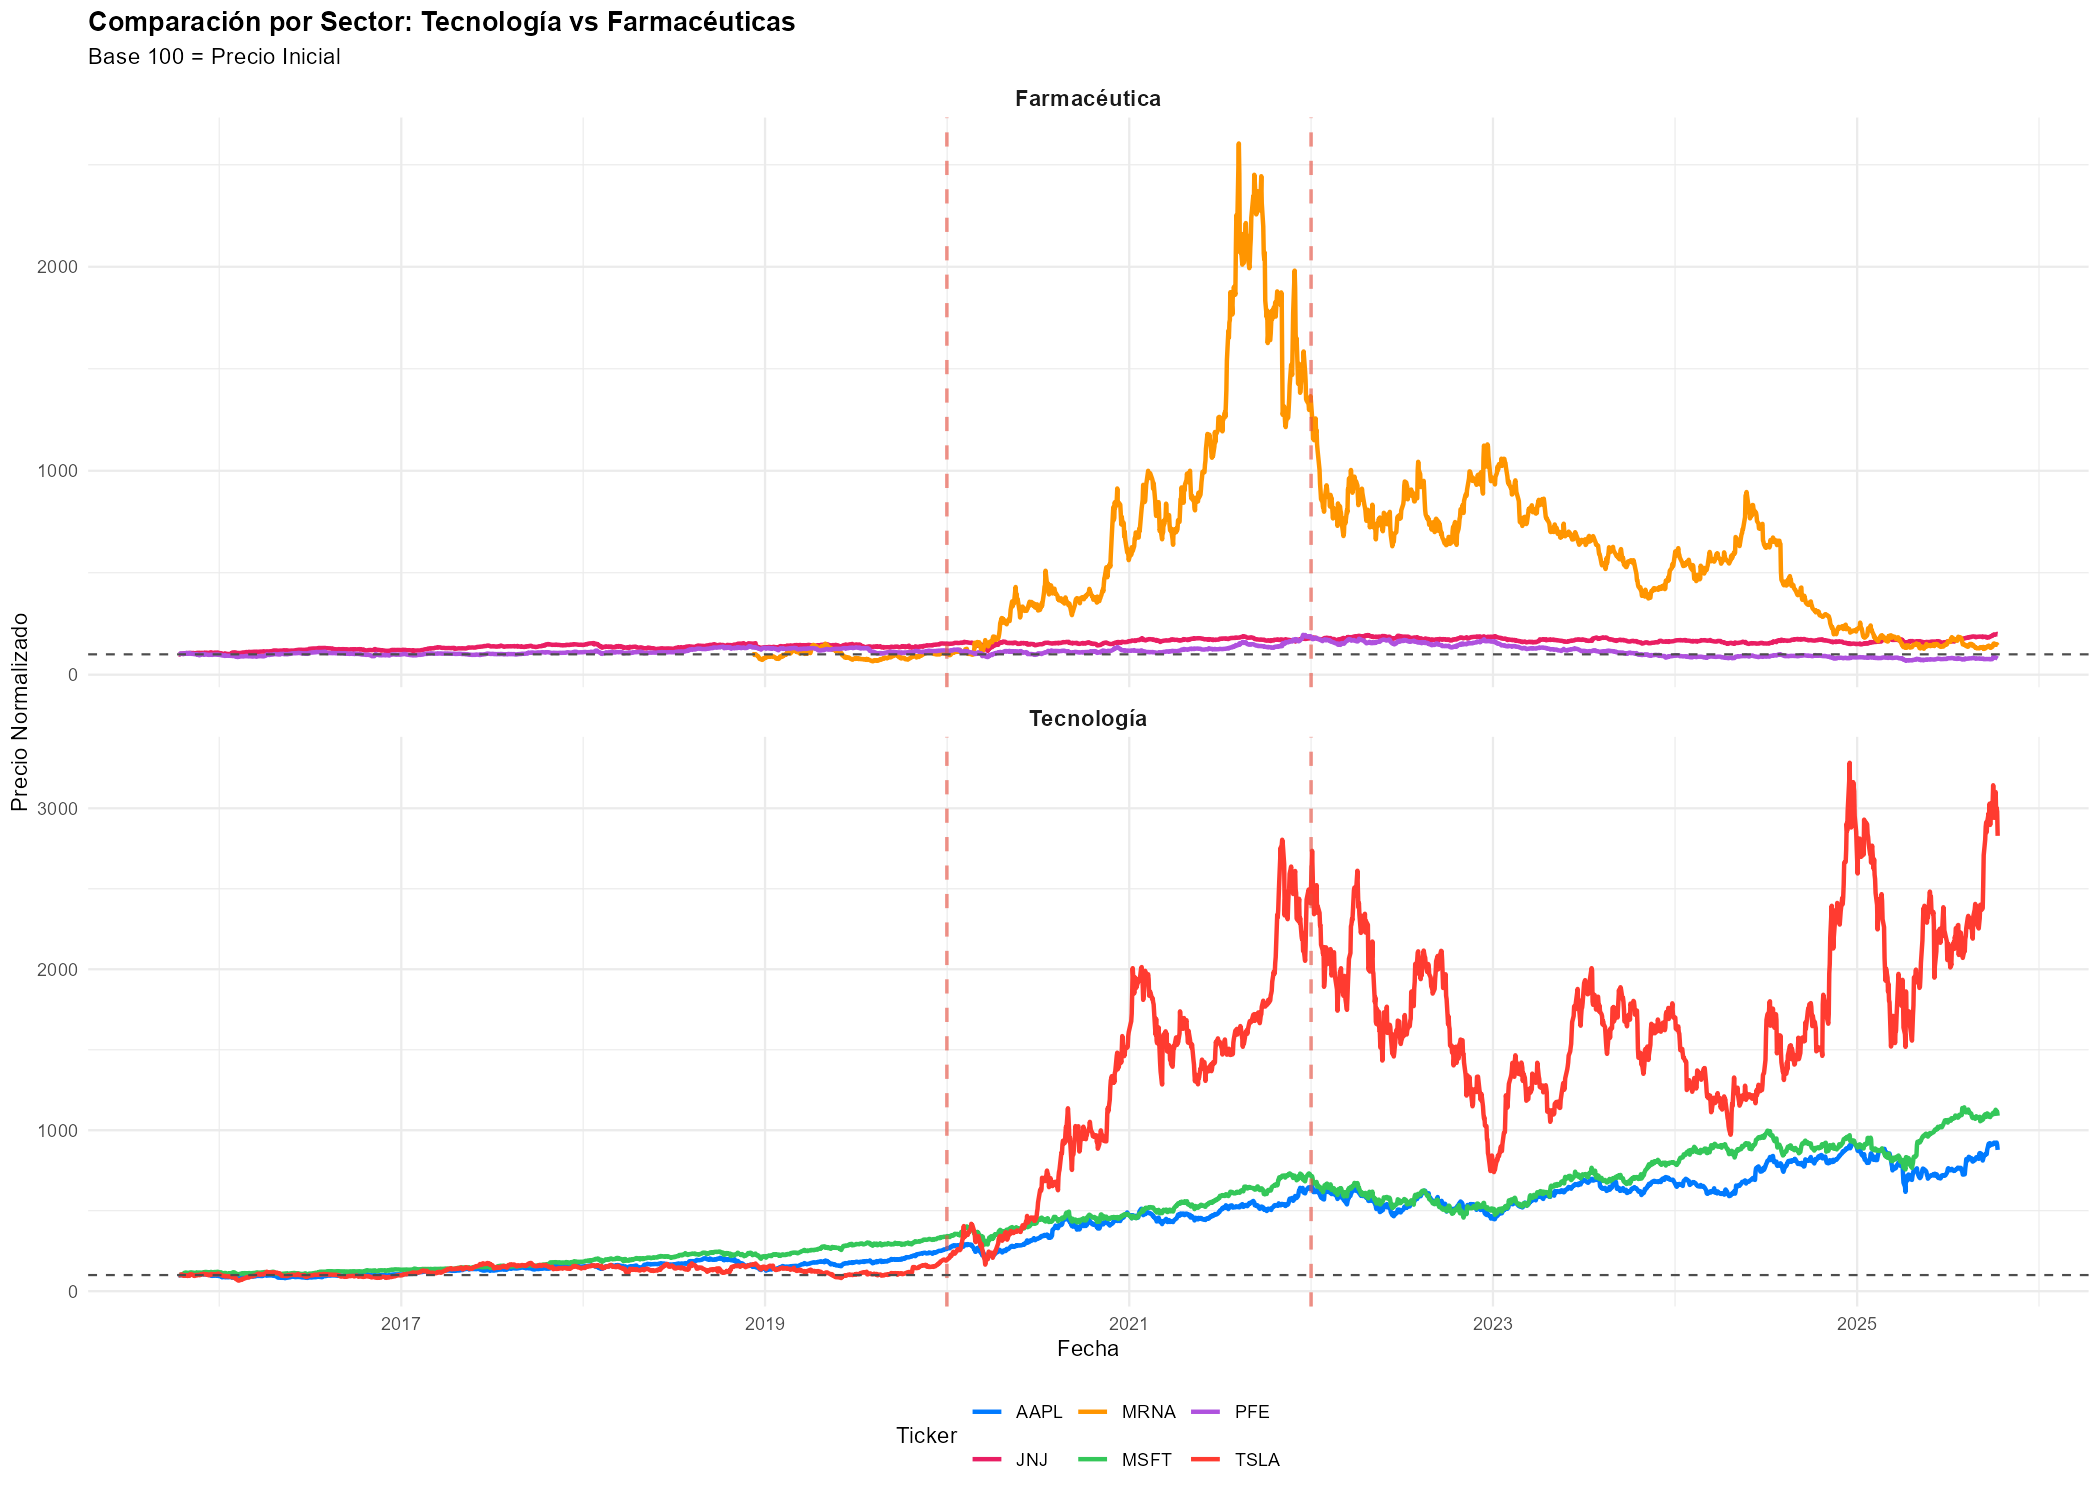
\includegraphics[width=1\linewidth]{graficos/03_comparacion_sector} \caption{Comparación de desempeño normalizado por sector. Panel superior: Farmacéuticas con Moderna mostrando crecimiento explosivo durante vacunas. Panel inferior: Tecnología con Tesla liderando los retornos. Líneas rojas verticales marcan el período COVID-19.}\label{fig:figura-sectores}
\end{figure}

La Figura 1 muestra el comportamiento diferenciado entre sectores. El sector tecnológico presenta crecimiento sostenido con Tesla liderando (+2,728\%), mientras que el farmacéutico muestra un pico en Moderna durante vacunas seguido de corrección. Este contraste será analizado en capítulos posteriores.

\section{Importancia del Pronóstico y Valor Agregado}\label{importancia-del-pronuxf3stico-y-valor-agregado}

\subsection{El Problema}\label{el-problema}

Los mercados financieros presentan comportamientos complejos que se intensifican durante crisis globales. El COVID-19 evidenció esto cuando los mercados experimentaron caídas abruptas, alta volatilidad y recuperaciones diferenciadas por sector. Los inversionistas y gestores de riesgo necesitan herramientas para anticipar movimientos de precios incluso en contextos de alta incertidumbre.

\subsection{El Valor Agregado}\label{el-valor-agregado}

Este proyecto analiza \textbf{series de tiempo de precios de acciones} durante un período de 10 años que incluye eventos extremos. El valor agregado reside en:

\textbf{1. Análisis con Datos Reales Abundantes:} Con 14,286 observaciones totales (2,514 por activo principal y 1,720 para MRNA), los análisis tienen suficiente poder estadístico para identificar patrones robustos, tendencias de largo plazo y quiebres estructurales.

\textbf{2. Múltiples Regímenes de Mercado:} El período analizado captura diferentes contextos de mercado, desde estabilidad pre-COVID hasta volatilidad extrema durante la pandemia (hasta 72\% anual en MRNA) y posterior normalización.

\textbf{3. Eventos Extremos Documentados:} El dataset incluye el crash de marzo 2020, el desarrollo de vacunas y la recuperación post-pandemia, permitiendo estudiar quiebres estructurales en series de tiempo y evaluar capacidad predictiva ante eventos de baja probabilidad pero alto impacto.

\textbf{4. Comparación Intersectorial Cuantificada:} Los datos revelan contrastes marcados:

\begin{itemize}
\tightlist
\item
  \textbf{Tecnología:} Retornos totales entre +777\% (AAPL) y +2,728\% (TSLA)
\item
  \textbf{Farmacéuticas:} Comportamiento heterogéneo desde -20\% (PFE) hasta +44\% (MRNA)
\item
  \textbf{Volatilidad:} Rango de 18\% (JNJ) hasta 72\% (MRNA)
\end{itemize}

\textbf{5. Caracterización Estadística:} Los datos permiten identificar propiedades como estacionariedad, autocorrelación, heterocedasticidad y cambios de régimen en volatilidad, aspectos que serán desarrollados en capítulos posteriores.

\textbf{6. Aplicación a Valoración de Opciones:} Los análisis de volatilidad histórica y comportamiento de precios se integran con el modelo Black-Scholes para mejorar la valoración de opciones financieras.

\section{Fuentes de Datos y Permisos de Uso}\label{fuentes-de-datos-y-permisos-de-uso}

\textbf{Fuente:} Yahoo Finance a través de la librería \texttt{quantmod} en R. Es una fuente pública reconocida en el sector financiero que permite acceso a datos históricos sin restricciones para uso académico y de investigación.

\textbf{Especificaciones técnicas:}

\begin{itemize}
\tightlist
\item
  \textbf{Período:} 2015-2025 (10 años, excepto MRNA que inicia en 2018)
\item
  \textbf{Observaciones totales:} 14,286 datos distribuidos en 6 activos
\item
  \textbf{Frecuencia:} Diaria (aproximadamente 252 días de trading por año)
\item
  \textbf{Acceso:} API pública sin permisos especiales requeridos
\item
  \textbf{Rango de precios:} Desde \$9.58 (TSLA mínimo) hasta \$535.64 (MSFT máximo)
\end{itemize}

\textbf{Variables recopiladas:}

\begin{itemize}
\tightlist
\item
  Precios: Cierre, apertura, máximo, mínimo (valores diarios en USD)
\item
  Volumen de negociación diario
\item
  Variables derivadas: Retornos diarios, retornos logarítmicos, volatilidad histórica
\item
  Clasificación temporal: Períodos COVID (Pre, Pandemia, Vacunas, Post)
\end{itemize}

\section{Impacto Esperado}\label{impacto-esperado}

El análisis de series de tiempo con más de 14,000 observaciones reales beneficia a:

\textbf{Inversionistas:} Comprensión documentada de cómo diferentes sectores responden a choques sistémicos, con evidencia cuantitativa de retornos y volatilidades observados durante crisis.

\textbf{Gestores de riesgo:} Identificación de patrones de volatilidad durante eventos extremos, con datos reales que muestran variaciones desde 18\% hasta 72\% de volatilidad anualizada según el activo y el período.

\textbf{Analistas financieros:} Caracterización cuantitativa de resiliencia sectorial respaldada por datos históricos de una década, incluyendo el evento más disruptivo de los mercados financieros en la última generación.

\textbf{Traders de opciones:} Estimación mejorada de volatilidad para valoración de derivados, con datos históricos que documentan cambios de régimen en volatilidad durante diferentes fases del mercado.

\textbf{Académicos:} Evidencia empírica robusta sobre comportamiento de series financieras durante crisis globales, con suficientes observaciones para análisis estadísticamente significativos y validación de modelos de series de tiempo.

\begin{center}\rule{0.5\linewidth}{0.5pt}\end{center}

\textbf{Nota:} Este documento constituye la propuesta inicial del proyecto. Los capítulos posteriores desarrollarán en detalle el análisis exploratorio de las series, pruebas de estacionariedad, modelado de volatilidad, identificación de quiebres estructurales y su integración con modelos de valoración de opciones financieras.

\chapter{Visualización de las Series de Tiempo}\label{intro}

Las visualizaciones tienen como objetivo explorar y comunicar los patrones, tendencias y comportamientos presentes en las series de tiempo de precios de acciones durante el período 2015-2025, con énfasis en el impacto del COVID-19.

\section{Series de Tiempo Completas}\label{series-de-tiempo-completas}

Los siguientes gráficos proporcionan una visión general de la evolución de los precios de cada activo a lo largo del período 2015-2025.

\subsection{Sector Tecnológico}\label{sector-tecnoluxf3gico}

\begin{figure}
\centering
\pandocbounded{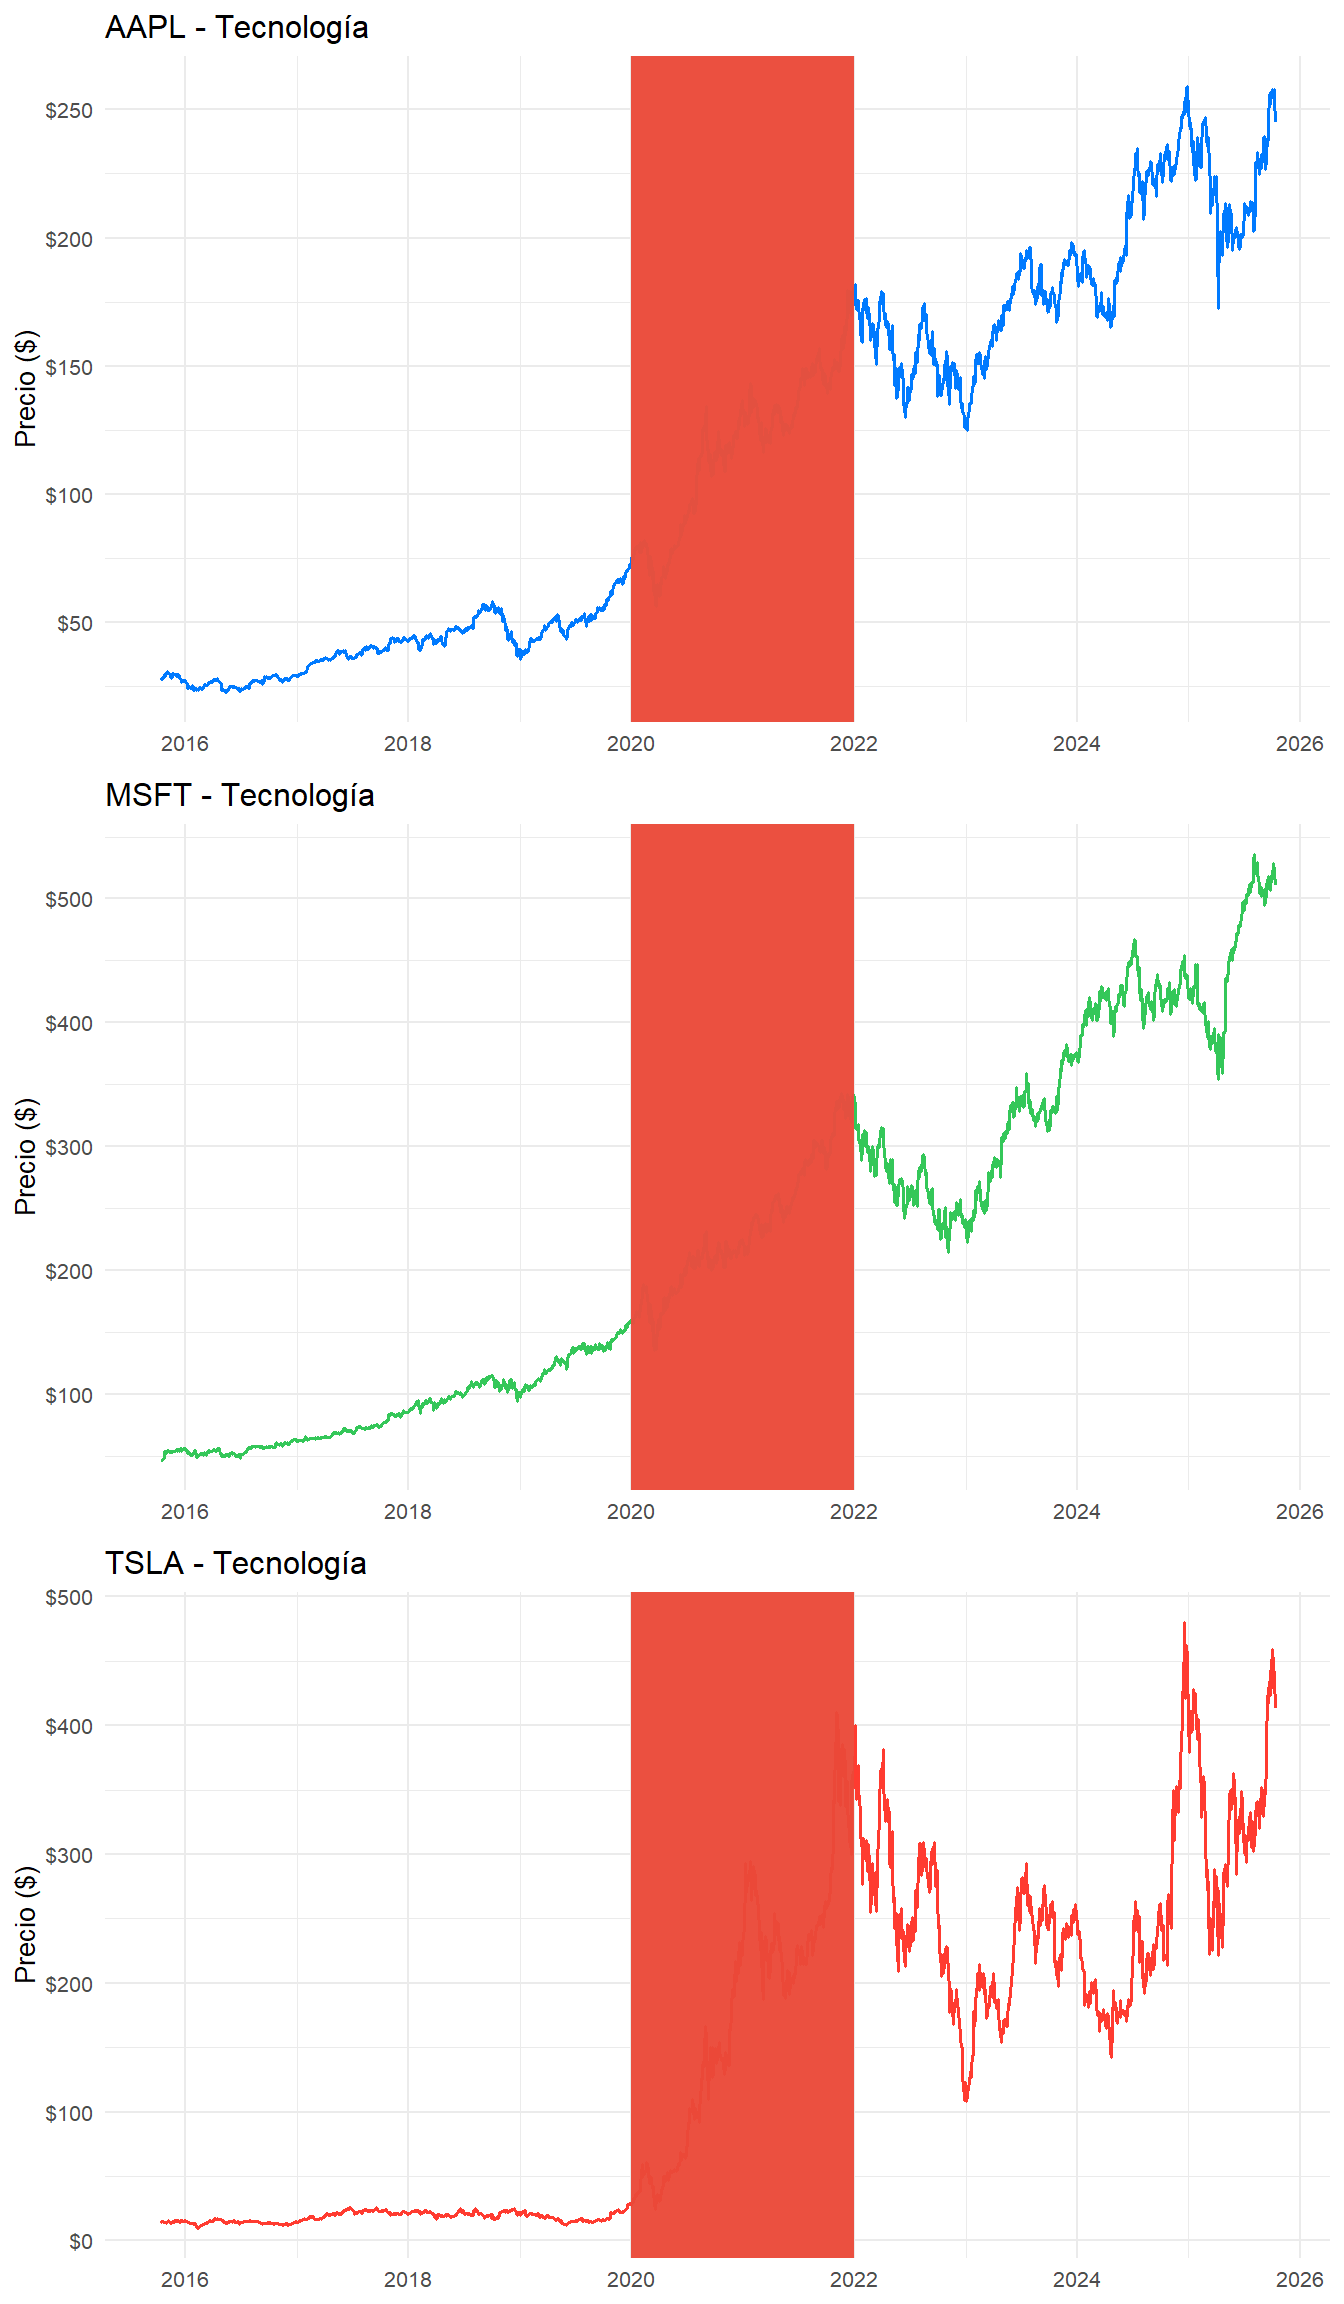
\includegraphics[keepaspectratio]{01-intro_files/figure-latex/series-tech-1.pdf}}
\caption{\label{fig:series-tech}Series de tiempo del sector tecnológico. Se observa el crecimiento explosivo de Tesla post-2019, la estabilidad relativa de Apple y Microsoft, y el impacto del COVID-19 (área sombreada) en las tres empresas.}
\end{figure}

\textbf{Observaciones clave del sector tecnológico:}

\begin{itemize}
\item
  \textbf{Apple (AAPL):} Muestra un crecimiento sostenido de \$22.58 a \$259.02 (+778\%), con volatilidad moderada (29.2\% anual). Durante el COVID-19, experimentó una caída breve seguida de recuperación acelerada.
\item
  \textbf{Microsoft (MSFT):} Presenta el comportamiento más estable del sector con crecimiento constante de \$46.68 a \$535.64 (+990\%). La volatilidad de 27\% anual es la más baja del sector tecnológico. Mínima afectación durante el crash de marzo 2020.
\item
  \textbf{Tesla (TSLA):} Exhibe el comportamiento más volátil (59.3\% anual) y el mayor retorno (+2,729\%). Se observa crecimiento casi exponencial desde 2019, con alta sensibilidad a eventos de mercado.
\end{itemize}

\subsection{Sector Farmacéutico}\label{sector-farmacuxe9utico}

\begin{figure}
\centering
\pandocbounded{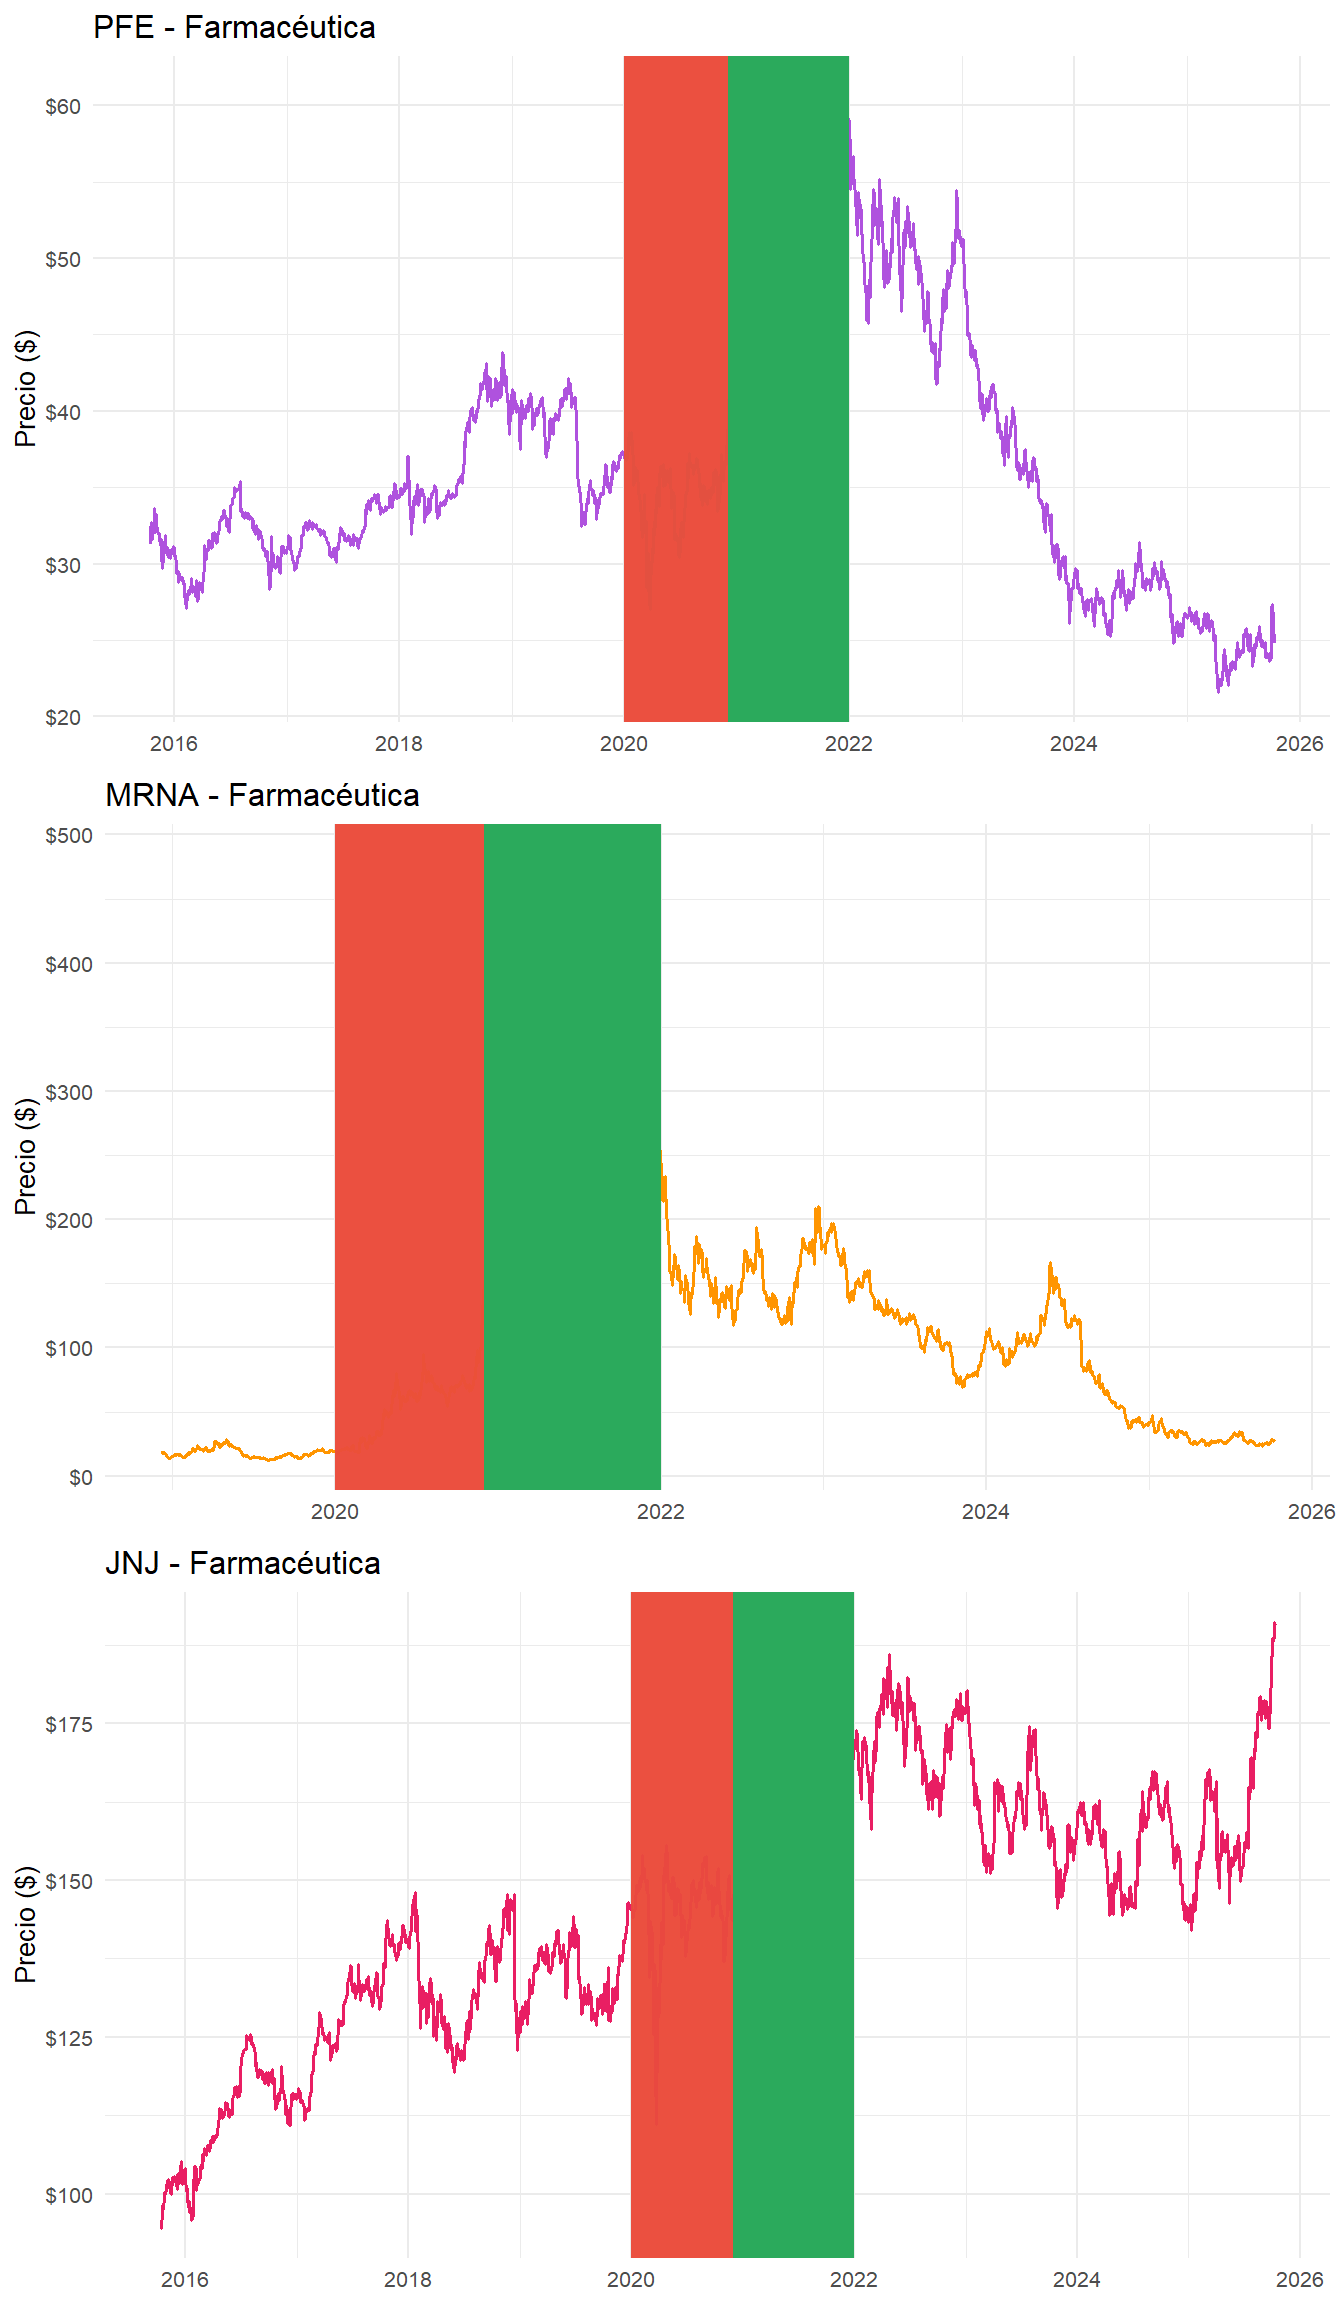
\includegraphics[keepaspectratio]{01-intro_files/figure-latex/series-pharma-1.pdf}}
\caption{\label{fig:series-pharma}Series de tiempo del sector farmacéutico. Destaca el pico dramático de Moderna durante el período de vacunas (2020-2021), mientras que Pfizer y J\&J muestran comportamientos más estables.}
\end{figure}

\textbf{Observaciones clave del sector farmacéutico:}

\begin{itemize}
\item
  \textbf{Pfizer (PFE):} Comportamiento estable con retorno negativo (-20.8\%). Volatilidad moderada (24\% anual). Pico durante el anuncio y distribución de vacunas, seguido de corrección.
\item
  \textbf{Moderna (MRNA):} La mayor volatilidad del dataset (72.1\% anual). Crecimiento explosivo durante el desarrollo de vacunas (diciembre 2020), alcanzando \$484.47 desde \$12.26. Posterior corrección drástica reflejando la normalización post-pandemia.
\item
  \textbf{Johnson \& Johnson (JNJ):} La menor volatilidad de todo el dataset (18.4\% anual). Comportamiento defensivo con retorno total de +99.8\%. Mínima afectación durante COVID-19.
\end{itemize}

\section{Análisis con Promedios Móviles}\label{anuxe1lisis-con-promedios-muxf3viles}

Los promedios móviles permiten suavizar la volatilidad diaria y visualizar tendencias subyacentes. Se calculan promedios de 7, 30 y 90 días.

\subsection{Promedios Móviles - Tecnología}\label{promedios-muxf3viles---tecnologuxeda}

\begin{verbatim}
## Warning: Removed 6 rows containing missing values or values outside the scale range
## (`geom_line()`).
\end{verbatim}

\begin{verbatim}
## Warning: Removed 29 rows containing missing values or values outside the scale range
## (`geom_line()`).
\end{verbatim}

\begin{verbatim}
## Warning: Removed 89 rows containing missing values or values outside the scale range
## (`geom_line()`).
\end{verbatim}

\begin{figure}
\centering
\pandocbounded{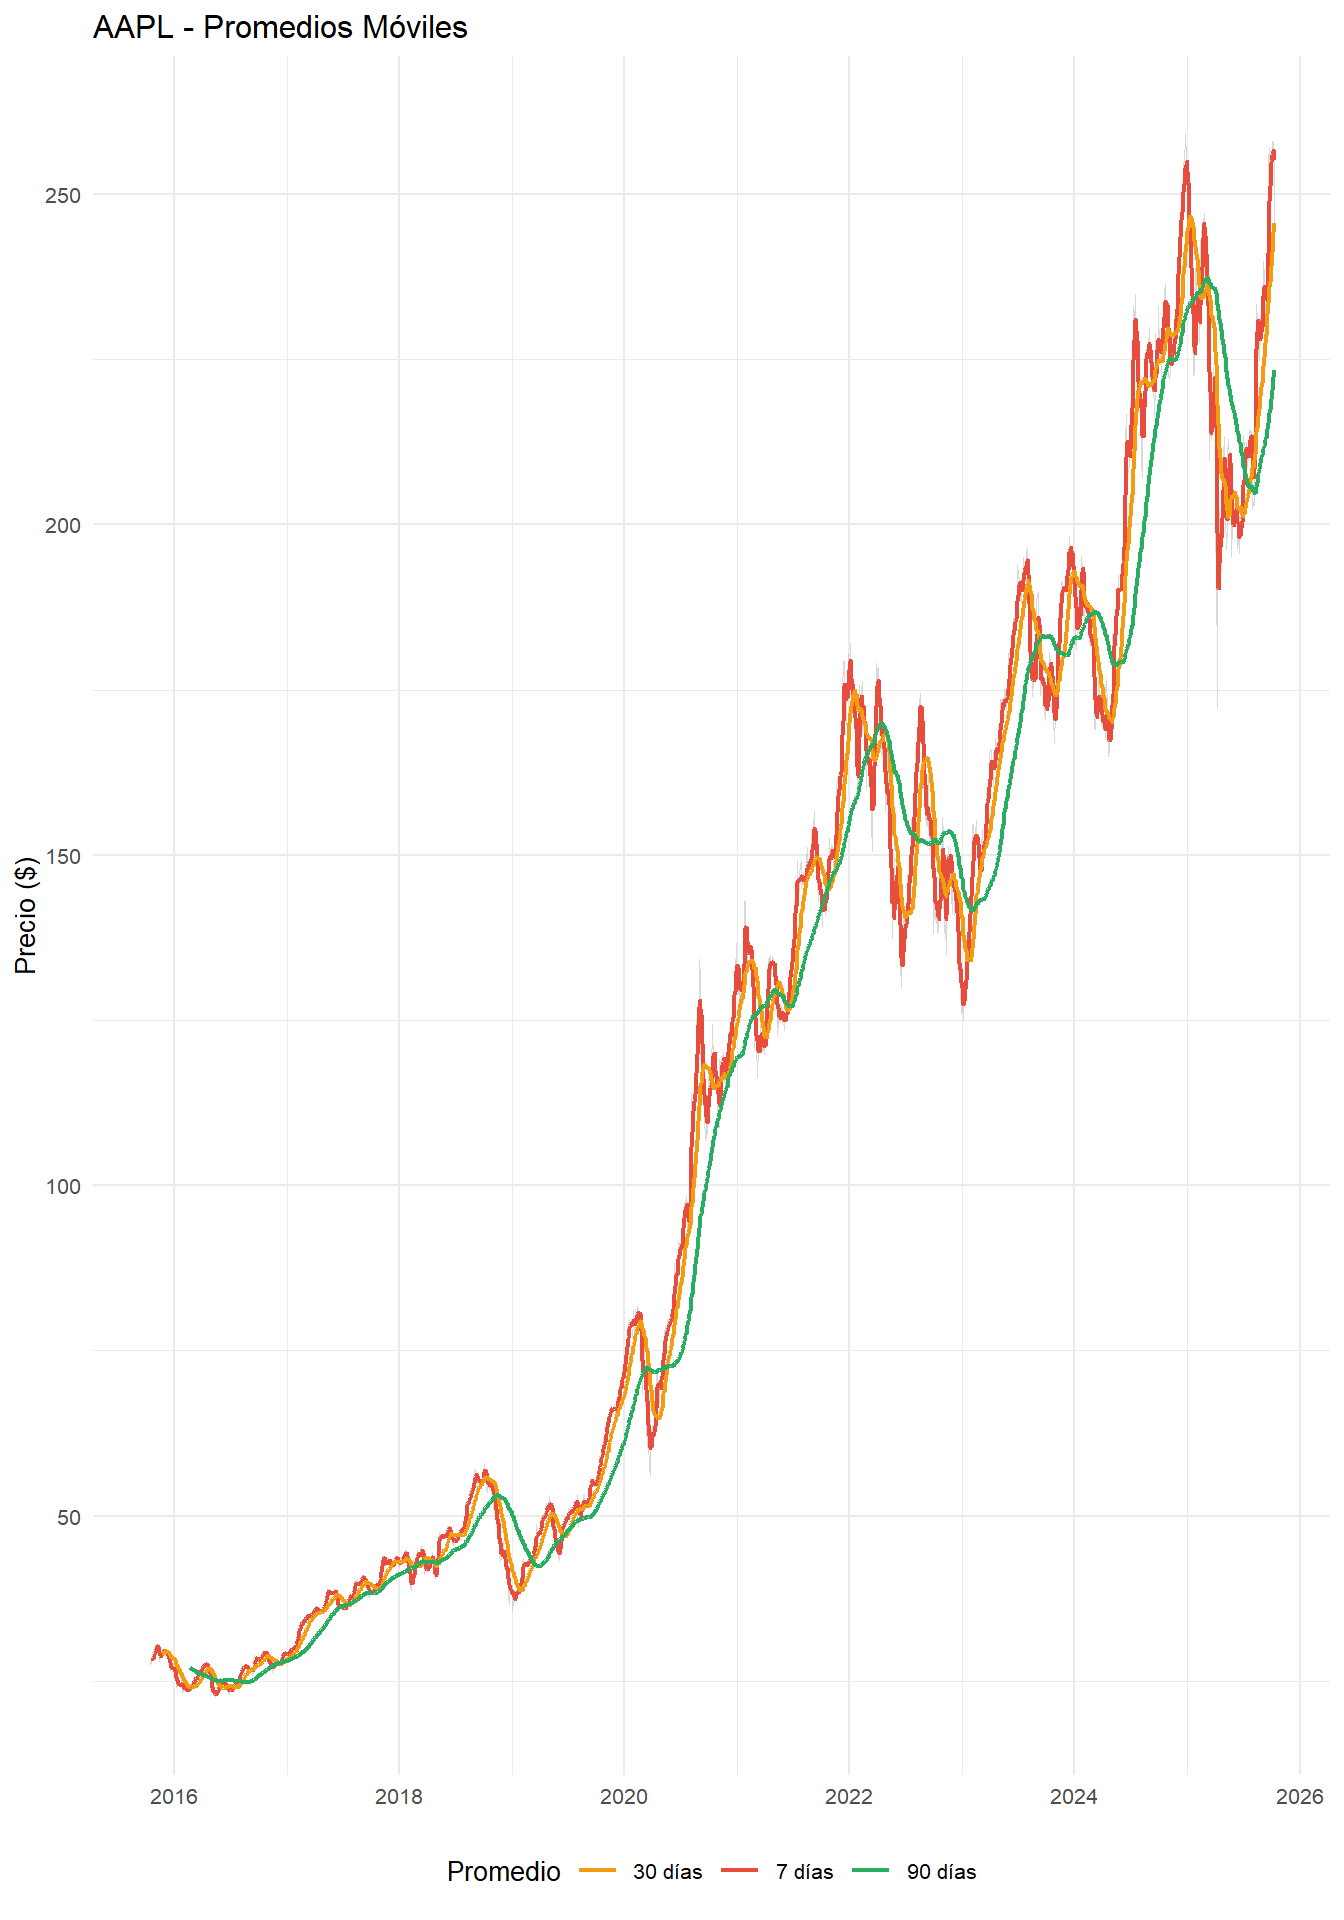
\includegraphics[keepaspectratio]{01-intro_files/figure-latex/sma-tech-1.pdf}}
\caption{\label{fig:sma-tech-1}Series con promedios móviles del sector tecnológico. Las líneas suavizadas (SMA 7, 30, 90 días) revelan las tendencias subyacentes y confirman el crecimiento sostenido post-COVID.}
\end{figure}

\begin{verbatim}
## Warning: Removed 6 rows containing missing values or values outside the scale range
## (`geom_line()`).
\end{verbatim}

\begin{verbatim}
## Warning: Removed 29 rows containing missing values or values outside the scale range
## (`geom_line()`).
\end{verbatim}

\begin{verbatim}
## Warning: Removed 89 rows containing missing values or values outside the scale range
## (`geom_line()`).
\end{verbatim}

\begin{figure}
\centering
\pandocbounded{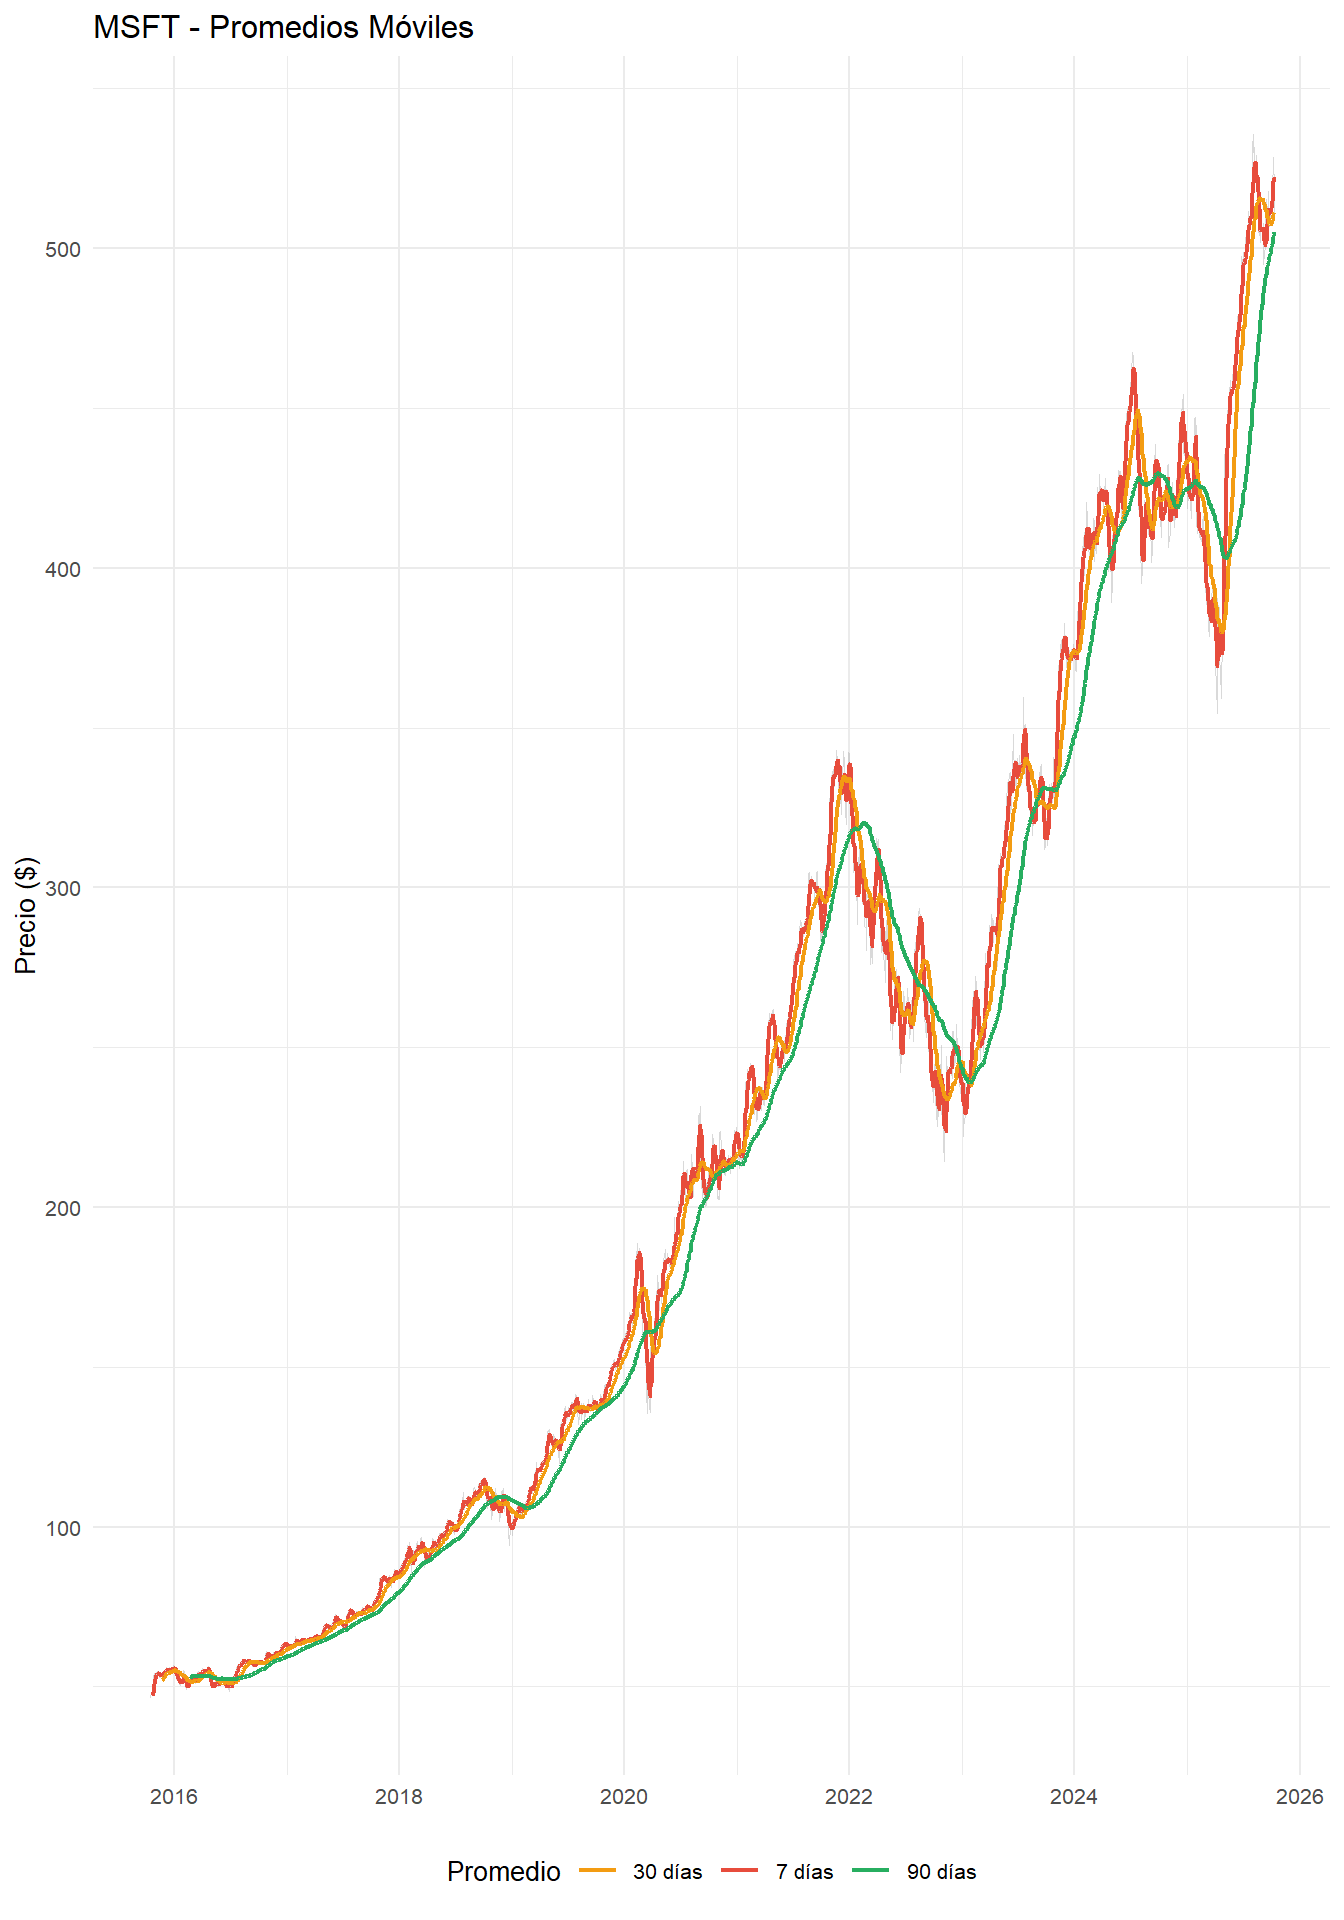
\includegraphics[keepaspectratio]{01-intro_files/figure-latex/sma-tech-2.pdf}}
\caption{\label{fig:sma-tech-2}Series con promedios móviles del sector tecnológico. Las líneas suavizadas (SMA 7, 30, 90 días) revelan las tendencias subyacentes y confirman el crecimiento sostenido post-COVID.}
\end{figure}

\begin{verbatim}
## Warning: Removed 6 rows containing missing values or values outside the scale range
## (`geom_line()`).
\end{verbatim}

\begin{verbatim}
## Warning: Removed 29 rows containing missing values or values outside the scale range
## (`geom_line()`).
\end{verbatim}

\begin{verbatim}
## Warning: Removed 89 rows containing missing values or values outside the scale range
## (`geom_line()`).
\end{verbatim}

\begin{figure}
\centering
\pandocbounded{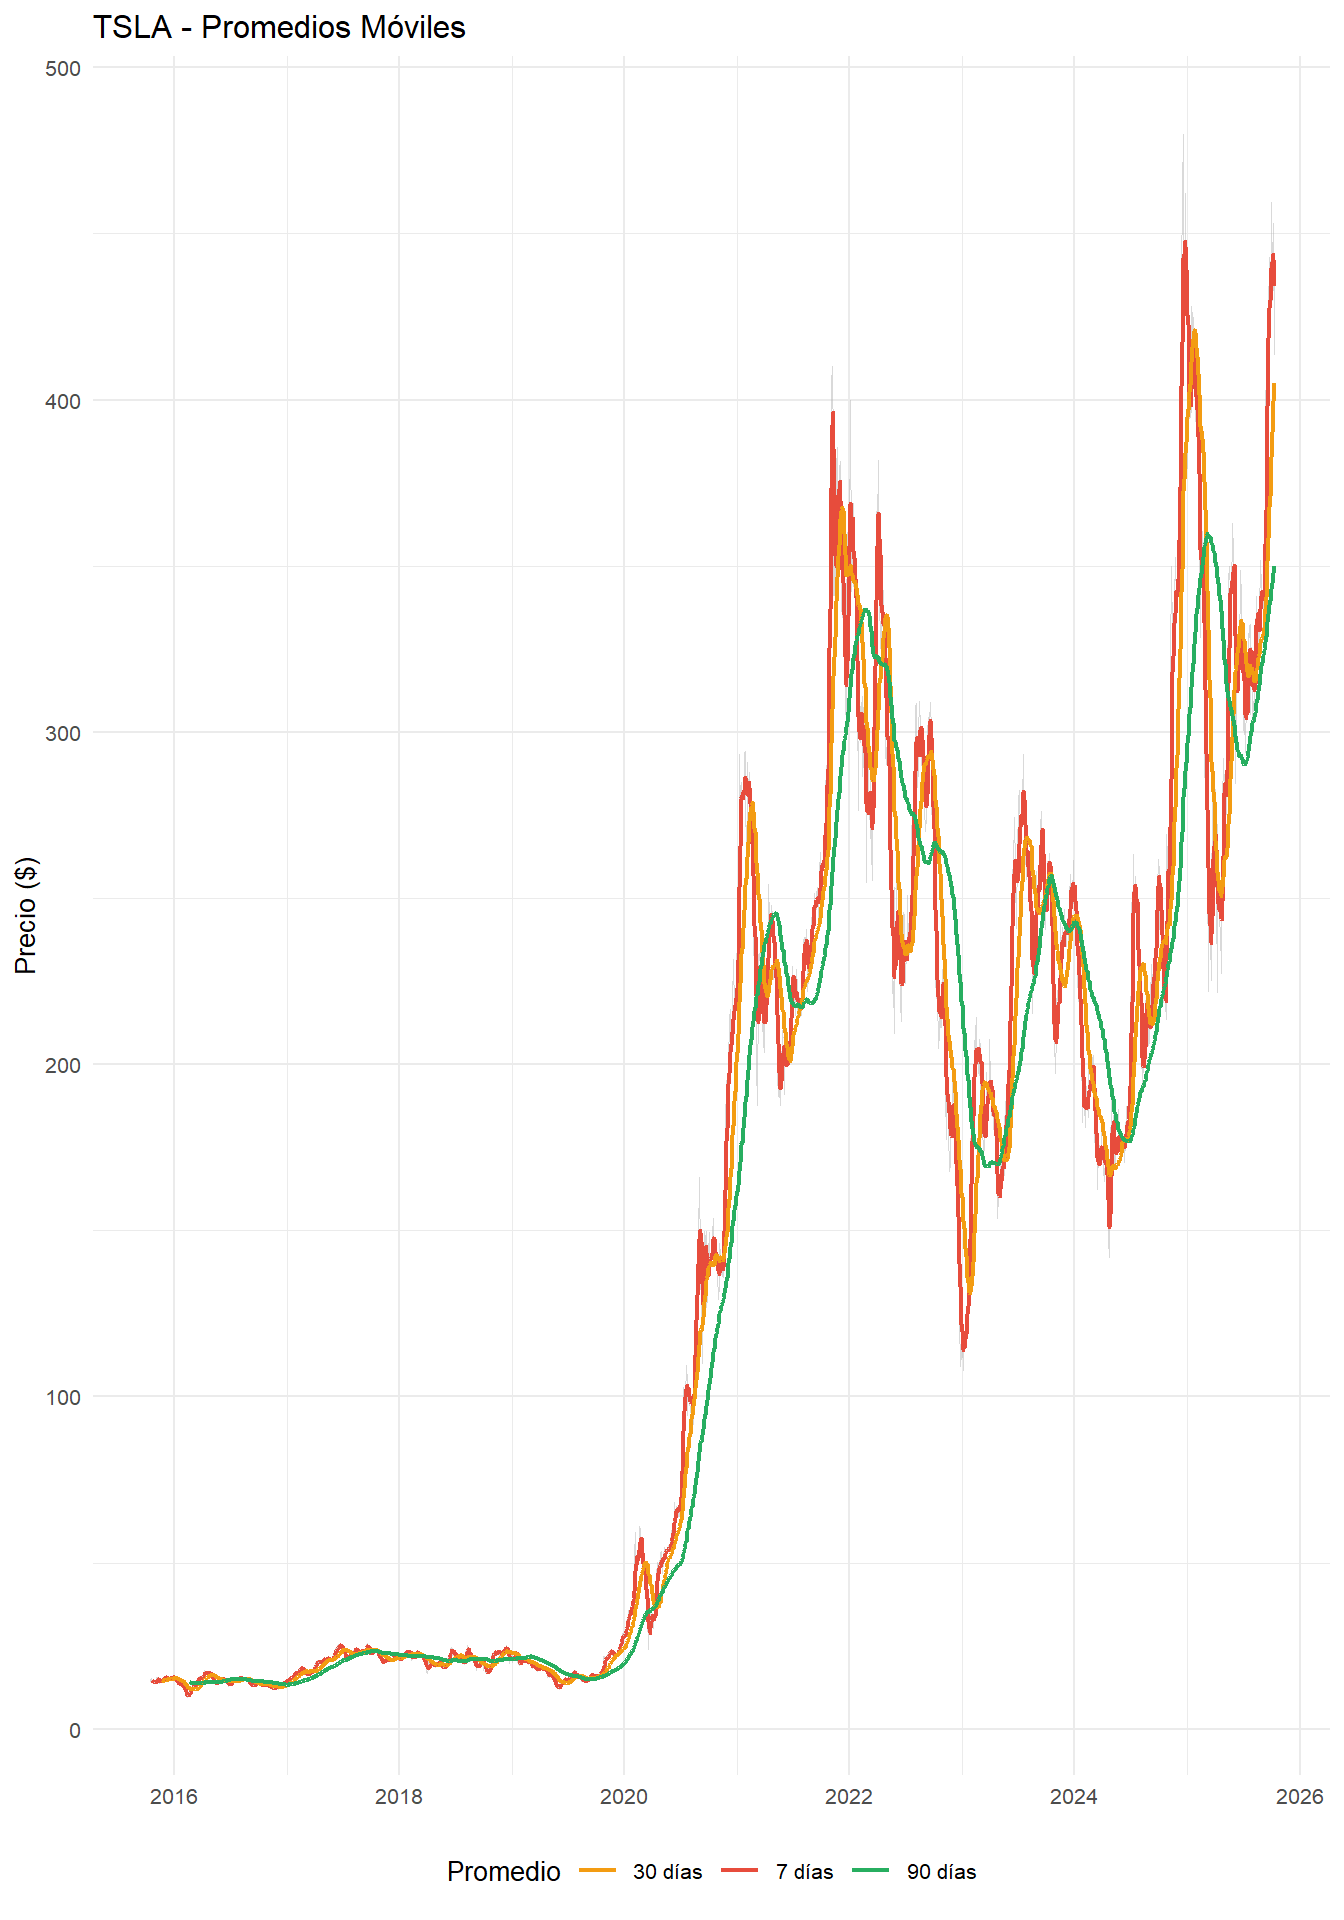
\includegraphics[keepaspectratio]{01-intro_files/figure-latex/sma-tech-3.pdf}}
\caption{\label{fig:sma-tech-3}Series con promedios móviles del sector tecnológico. Las líneas suavizadas (SMA 7, 30, 90 días) revelan las tendencias subyacentes y confirman el crecimiento sostenido post-COVID.}
\end{figure}

\textbf{Interpretación de promedios móviles:}

\begin{itemize}
\tightlist
\item
  \textbf{SMA 7 días:} Reacciona rápidamente a cambios, útil para identificar reversiones de corto plazo.
\item
  \textbf{SMA 30 días:} Revela tendencias de mediano plazo, filtrando ruido diario.
\item
  \textbf{SMA 90 días:} Muestra la tendencia de largo plazo, especialmente útil para identificar cambios de régimen durante COVID-19.
\end{itemize}

\subsection{Promedios Móviles - Farmacéuticas}\label{promedios-muxf3viles---farmacuxe9uticas}

\begin{verbatim}
## Warning: Removed 6 rows containing missing values or values outside the scale range
## (`geom_line()`).
\end{verbatim}

\begin{verbatim}
## Warning: Removed 29 rows containing missing values or values outside the scale range
## (`geom_line()`).
\end{verbatim}

\begin{verbatim}
## Warning: Removed 89 rows containing missing values or values outside the scale range
## (`geom_line()`).
\end{verbatim}

\begin{figure}
\centering
\pandocbounded{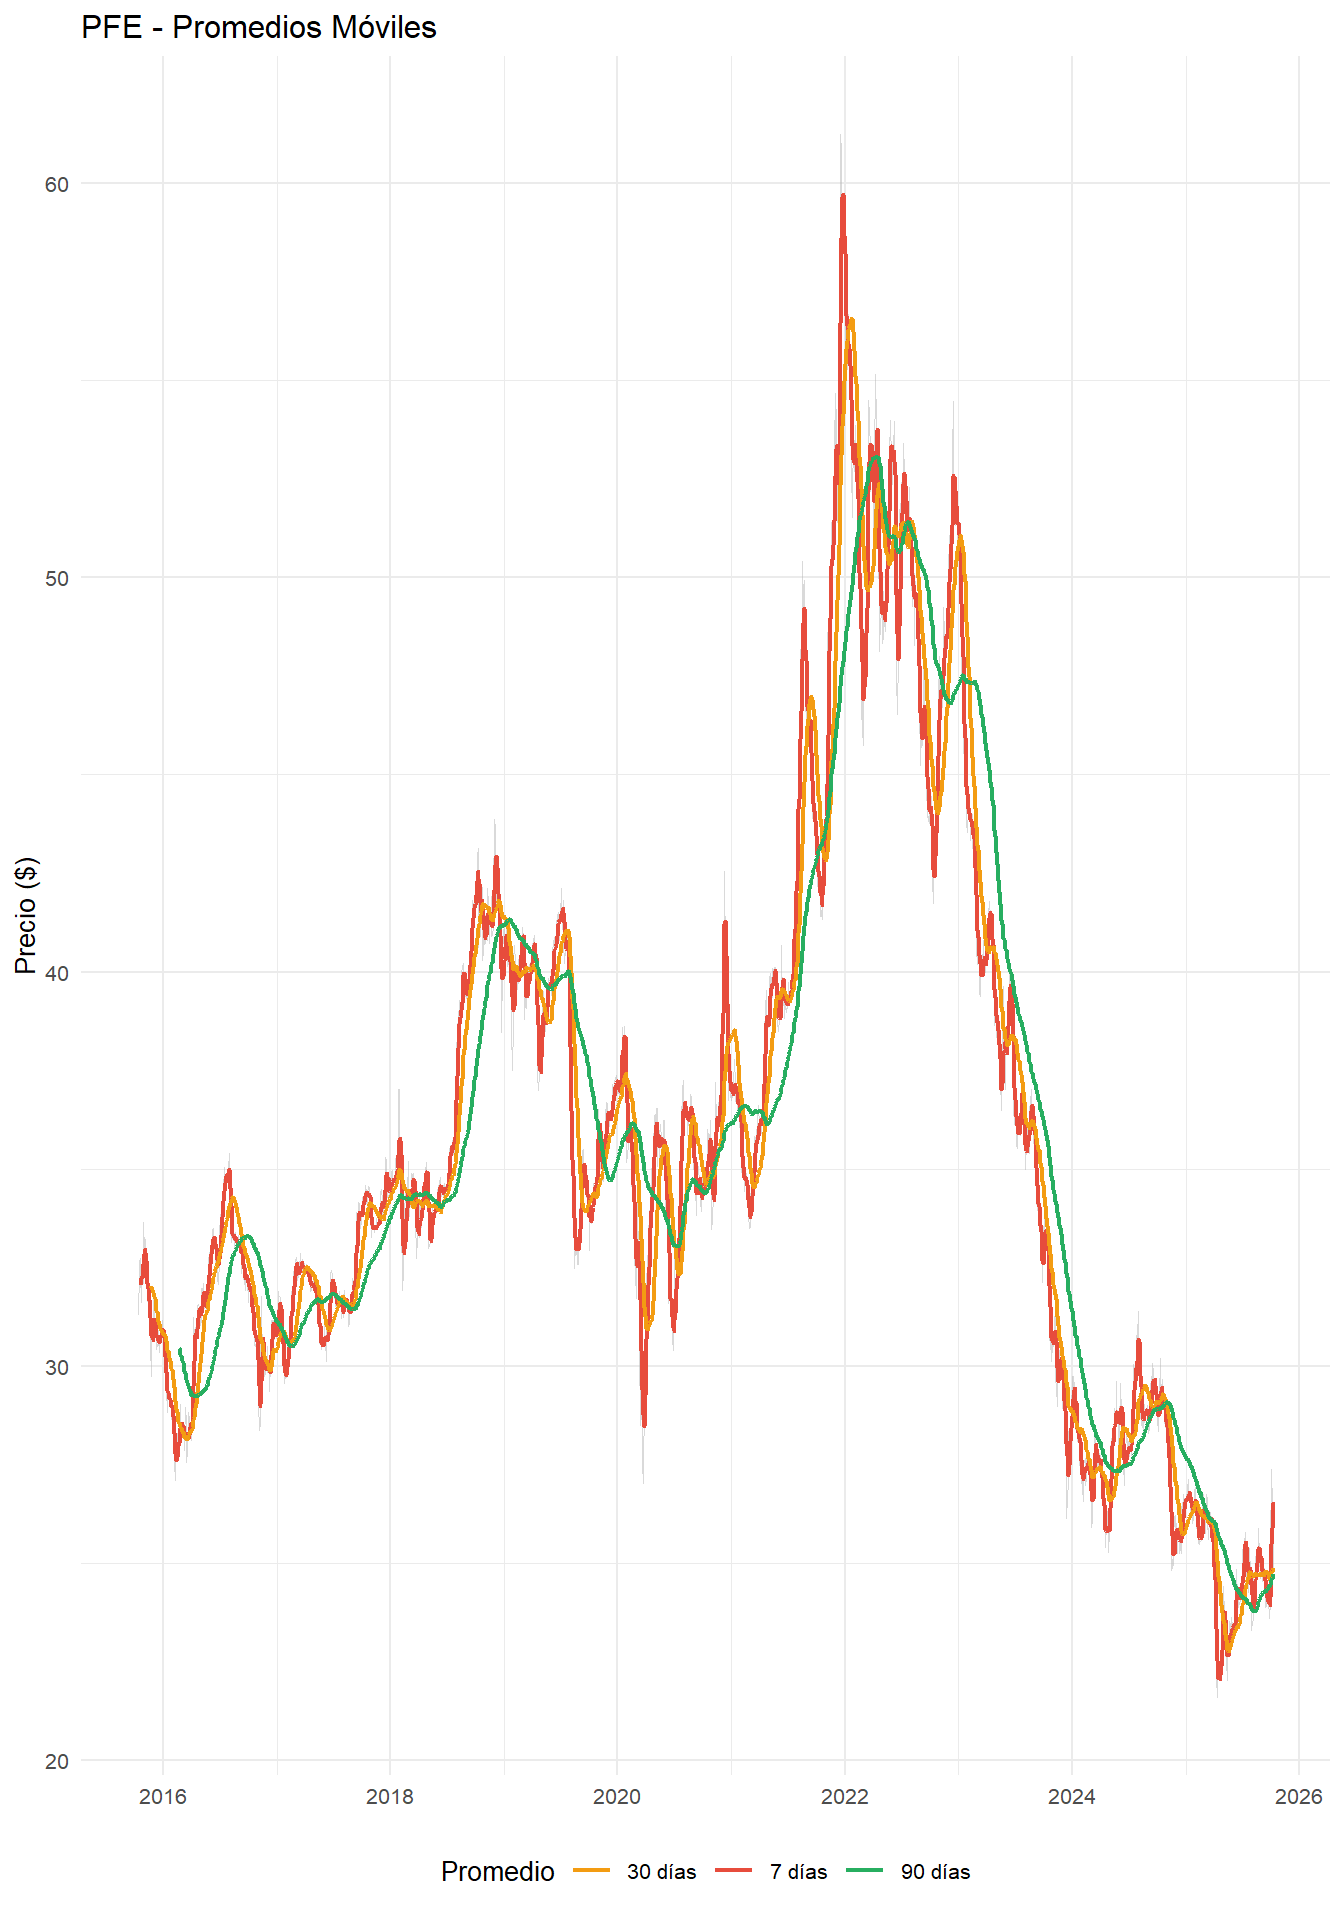
\includegraphics[keepaspectratio]{01-intro_files/figure-latex/sma-pharma-1.pdf}}
\caption{\label{fig:sma-pharma-1}Series con promedios móviles del sector farmacéutico. El caso de Moderna es particularmente interesante, mostrando cómo los promedios capturan el ciclo completo de auge y corrección.}
\end{figure}

\begin{verbatim}
## Warning: Removed 6 rows containing missing values or values outside the scale range
## (`geom_line()`).
\end{verbatim}

\begin{verbatim}
## Warning: Removed 29 rows containing missing values or values outside the scale range
## (`geom_line()`).
\end{verbatim}

\begin{verbatim}
## Warning: Removed 89 rows containing missing values or values outside the scale range
## (`geom_line()`).
\end{verbatim}

\begin{figure}
\centering
\pandocbounded{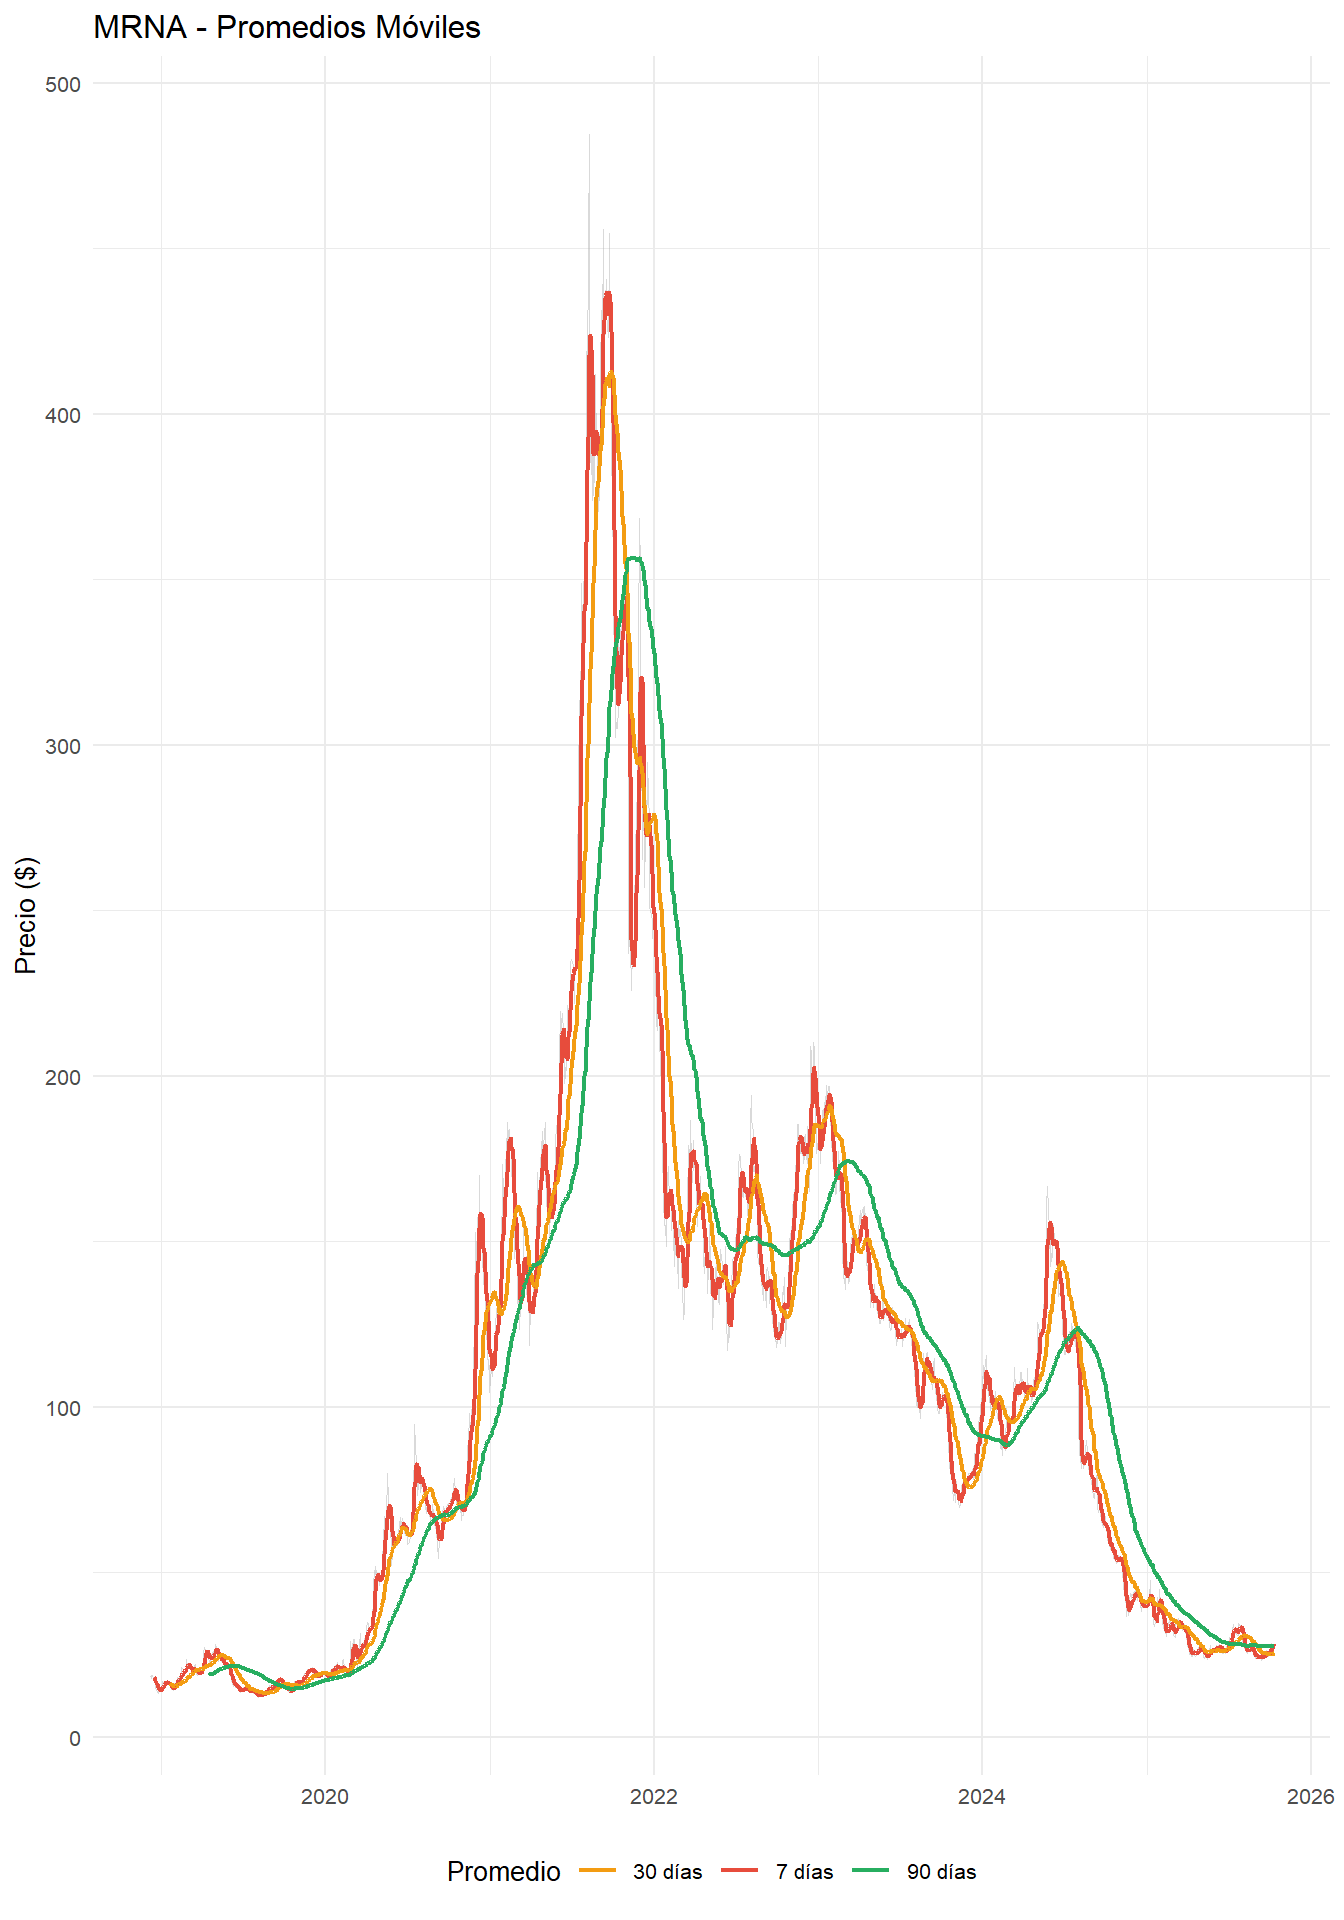
\includegraphics[keepaspectratio]{01-intro_files/figure-latex/sma-pharma-2.pdf}}
\caption{\label{fig:sma-pharma-2}Series con promedios móviles del sector farmacéutico. El caso de Moderna es particularmente interesante, mostrando cómo los promedios capturan el ciclo completo de auge y corrección.}
\end{figure}

\begin{verbatim}
## Warning: Removed 6 rows containing missing values or values outside the scale range
## (`geom_line()`).
\end{verbatim}

\begin{verbatim}
## Warning: Removed 29 rows containing missing values or values outside the scale range
## (`geom_line()`).
\end{verbatim}

\begin{verbatim}
## Warning: Removed 89 rows containing missing values or values outside the scale range
## (`geom_line()`).
\end{verbatim}

\begin{figure}
\centering
\pandocbounded{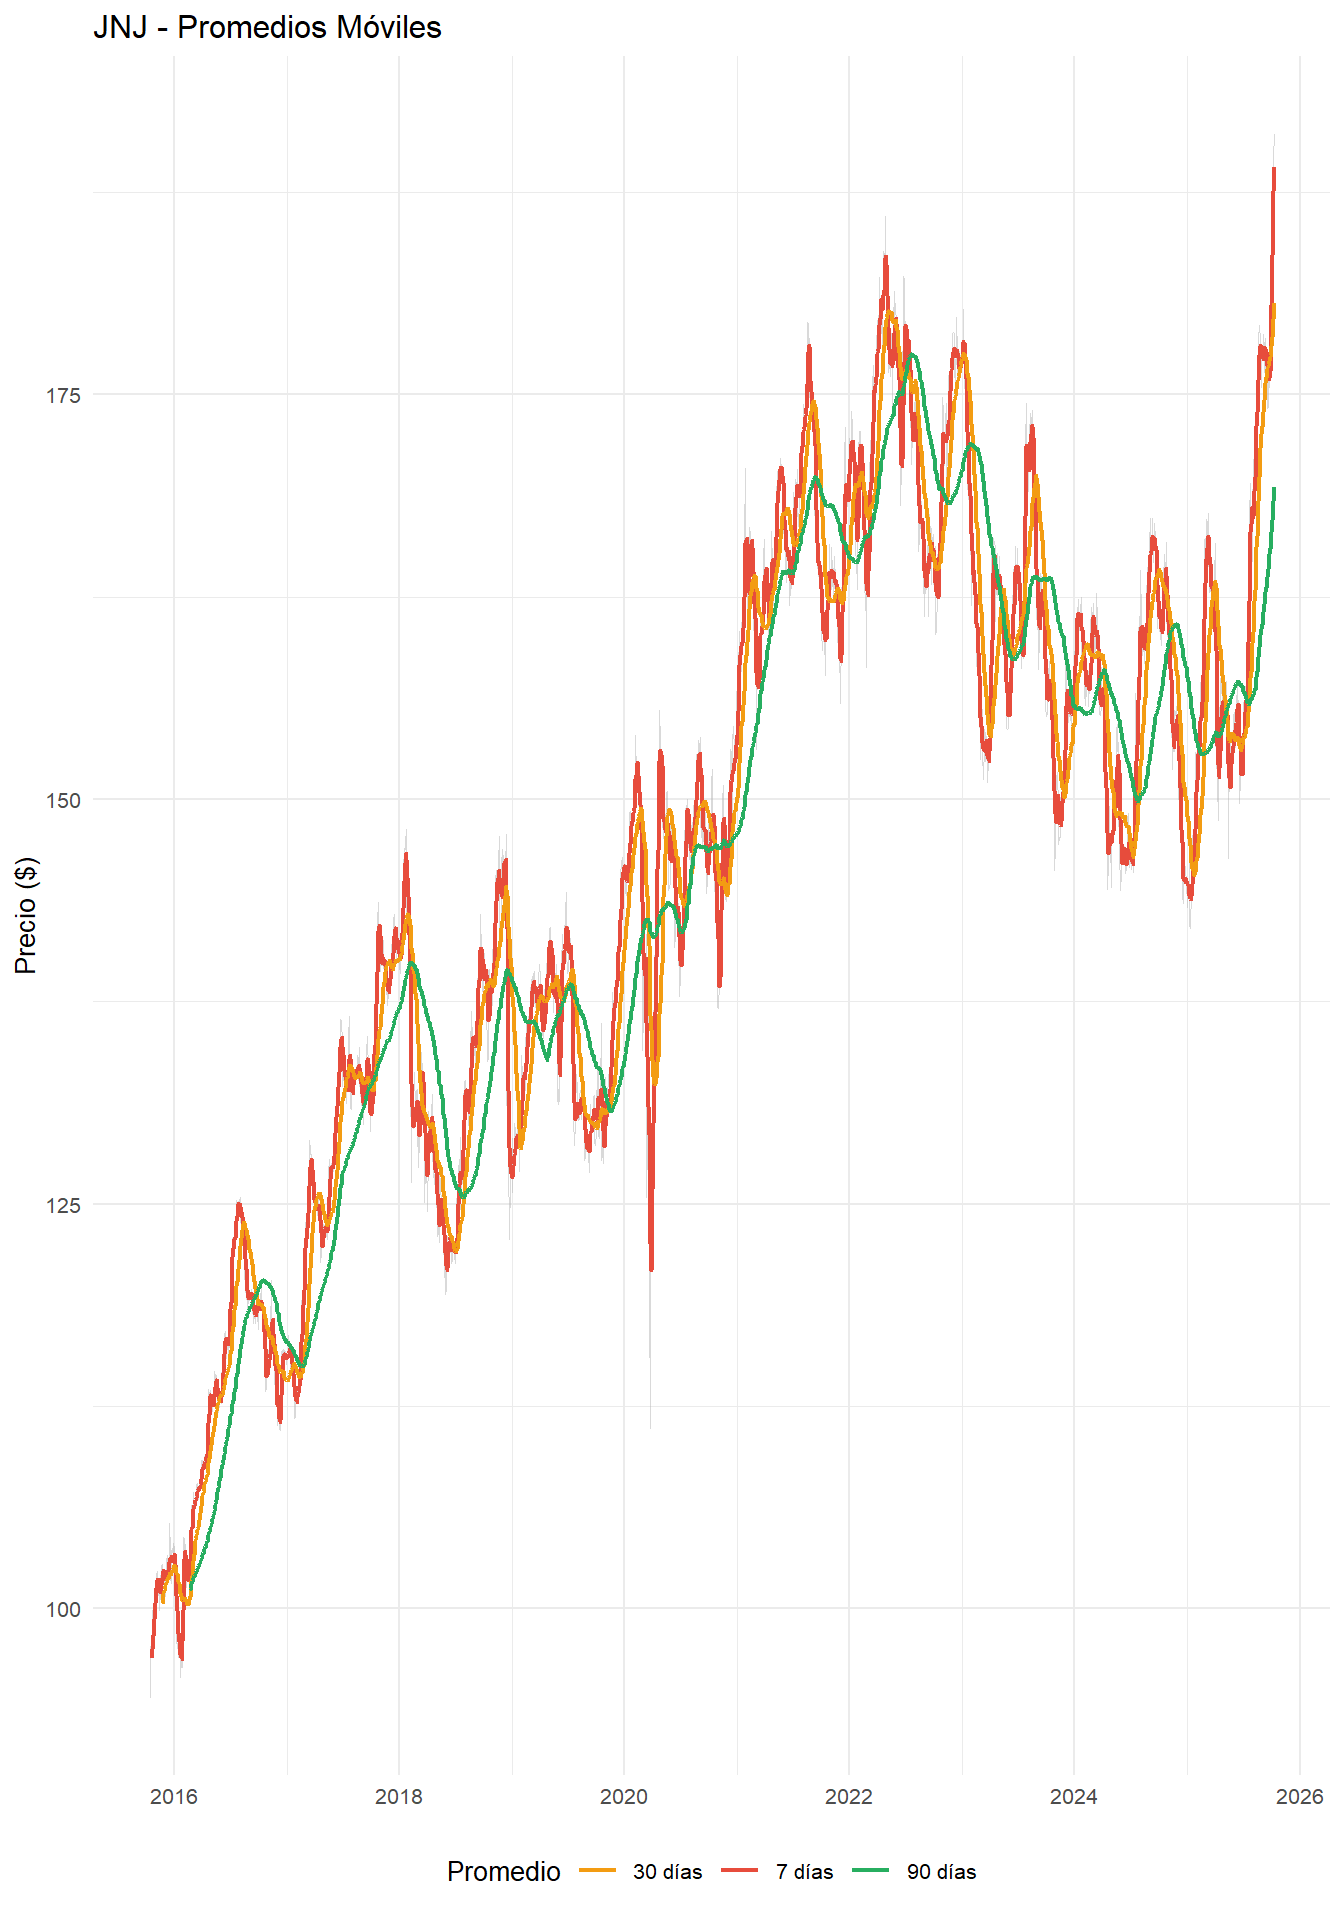
\includegraphics[keepaspectratio]{01-intro_files/figure-latex/sma-pharma-3.pdf}}
\caption{\label{fig:sma-pharma-3}Series con promedios móviles del sector farmacéutico. El caso de Moderna es particularmente interesante, mostrando cómo los promedios capturan el ciclo completo de auge y corrección.}
\end{figure}

\section{Análisis de Rezagos}\label{anuxe1lisis-de-rezagos}

Los gráficos de rezago permiten identificar dependencia temporal en las series, evaluando si el precio de hoy está correlacionado con el precio de días anteriores.

\begin{verbatim}
## Warning: Removed 1 row containing missing values or values outside the scale range
## (`geom_point()`).
\end{verbatim}

\begin{verbatim}
## Warning: Removed 7 rows containing missing values or values outside the scale range
## (`geom_point()`).
\end{verbatim}

\begin{verbatim}
## Warning: Removed 1 row containing missing values or values outside the scale range
## (`geom_point()`).
\end{verbatim}

\begin{verbatim}
## Warning: Removed 7 rows containing missing values or values outside the scale range
## (`geom_point()`).
\end{verbatim}

\begin{verbatim}
## Warning: Removed 1 row containing missing values or values outside the scale range
## (`geom_point()`).
\end{verbatim}

\begin{verbatim}
## Warning: Removed 7 rows containing missing values or values outside the scale range
## (`geom_point()`).
\end{verbatim}

\begin{figure}
\centering
\pandocbounded{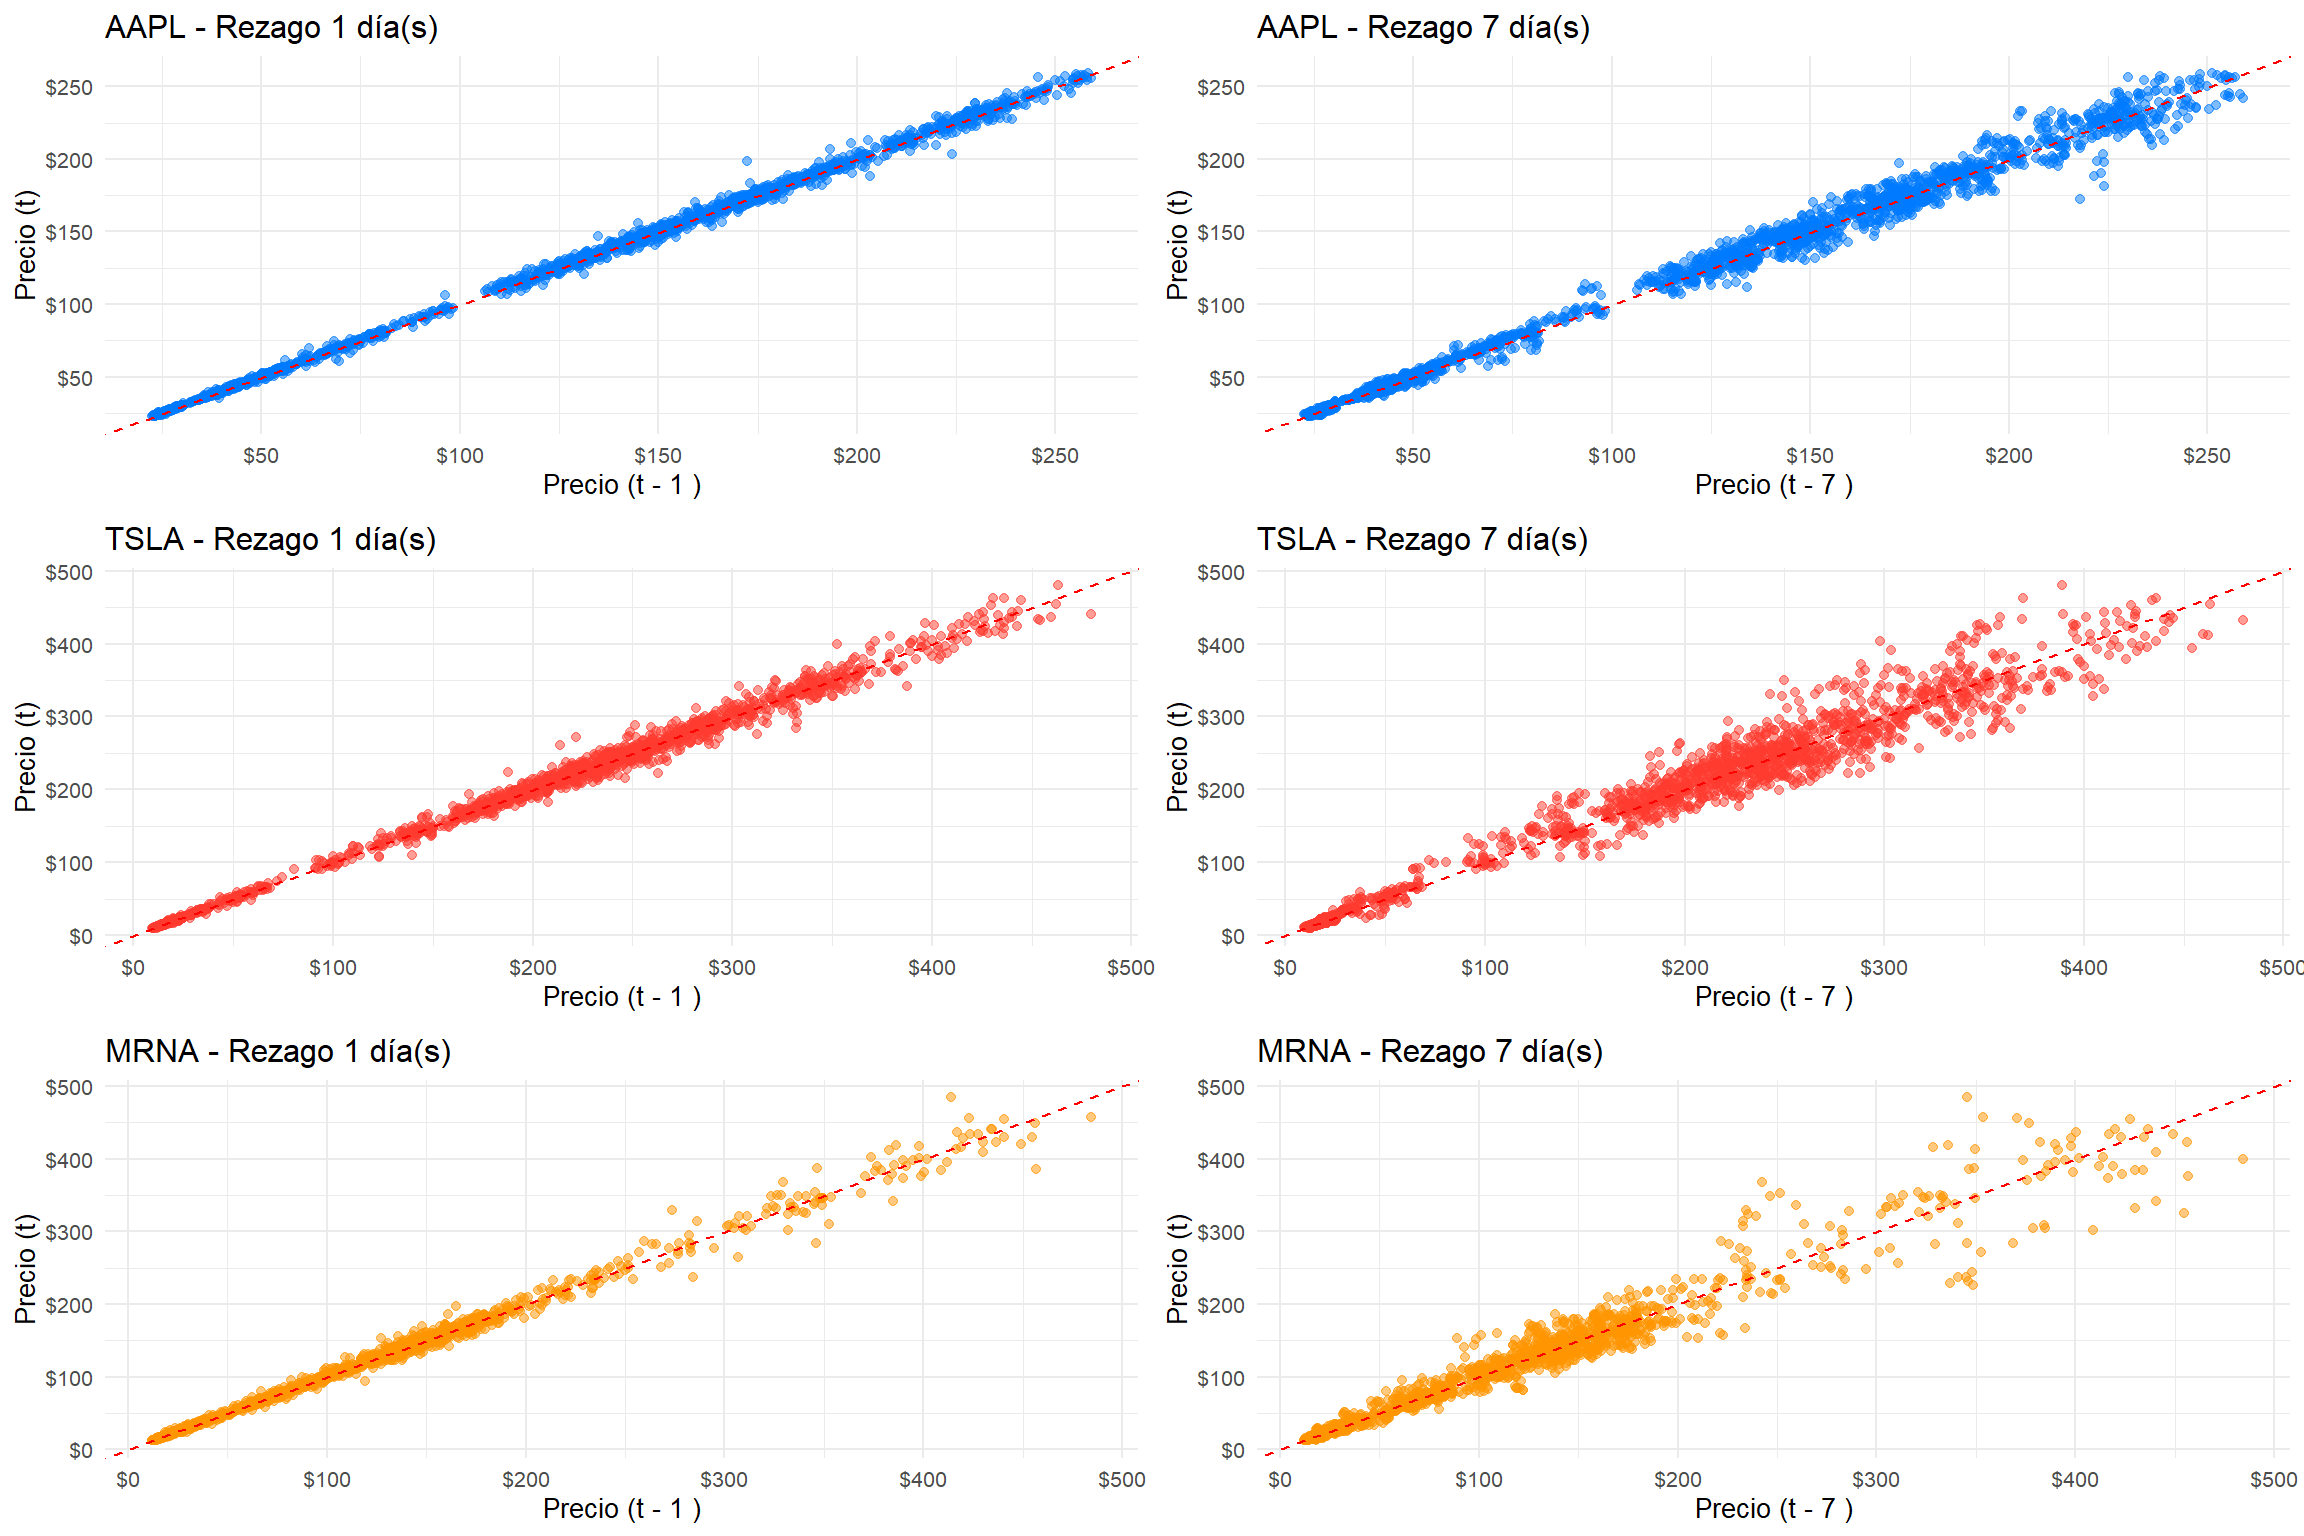
\includegraphics[keepaspectratio]{01-intro_files/figure-latex/lag-plots-1.pdf}}
\caption{\label{fig:lag-plots}Gráficos de rezago para lag 1 y lag 7 días. La concentración de puntos en la diagonal sugiere autocorrelación positiva, especialmente en lag 1.}
\end{figure}

\textbf{Interpretación de rezagos:}

\begin{itemize}
\item
  \textbf{Lag 1 (día anterior):} La mayoría de los puntos se concentran cerca de la diagonal, indicando autocorrelación positiva débil. Los precios tienden a persistir de un día al siguiente, especialmente en niveles bajos y altos.
\item
  \textbf{Lag 7 (semana anterior):} Mayor dispersión que lag 1, sugiriendo autocorrelación semanal muy débil. Las ventas de un día específico no predicen confiablemente el mismo día de la semana siguiente, excepto en valores extremos.
\item
  \textbf{Observación sectorial:} Tesla y Moderna muestran mayor dispersión debido a su alta volatilidad, mientras que activos más estables como J\&J presentan patrones más concentrados.
\end{itemize}

\section{Estacionalidad Anual}\label{estacionalidad-anual}

El análisis de estacionalidad revela patrones recurrentes a lo largo del año calendario, particularmente relevantes durante el período COVID-19.

\begin{figure}
\centering
\pandocbounded{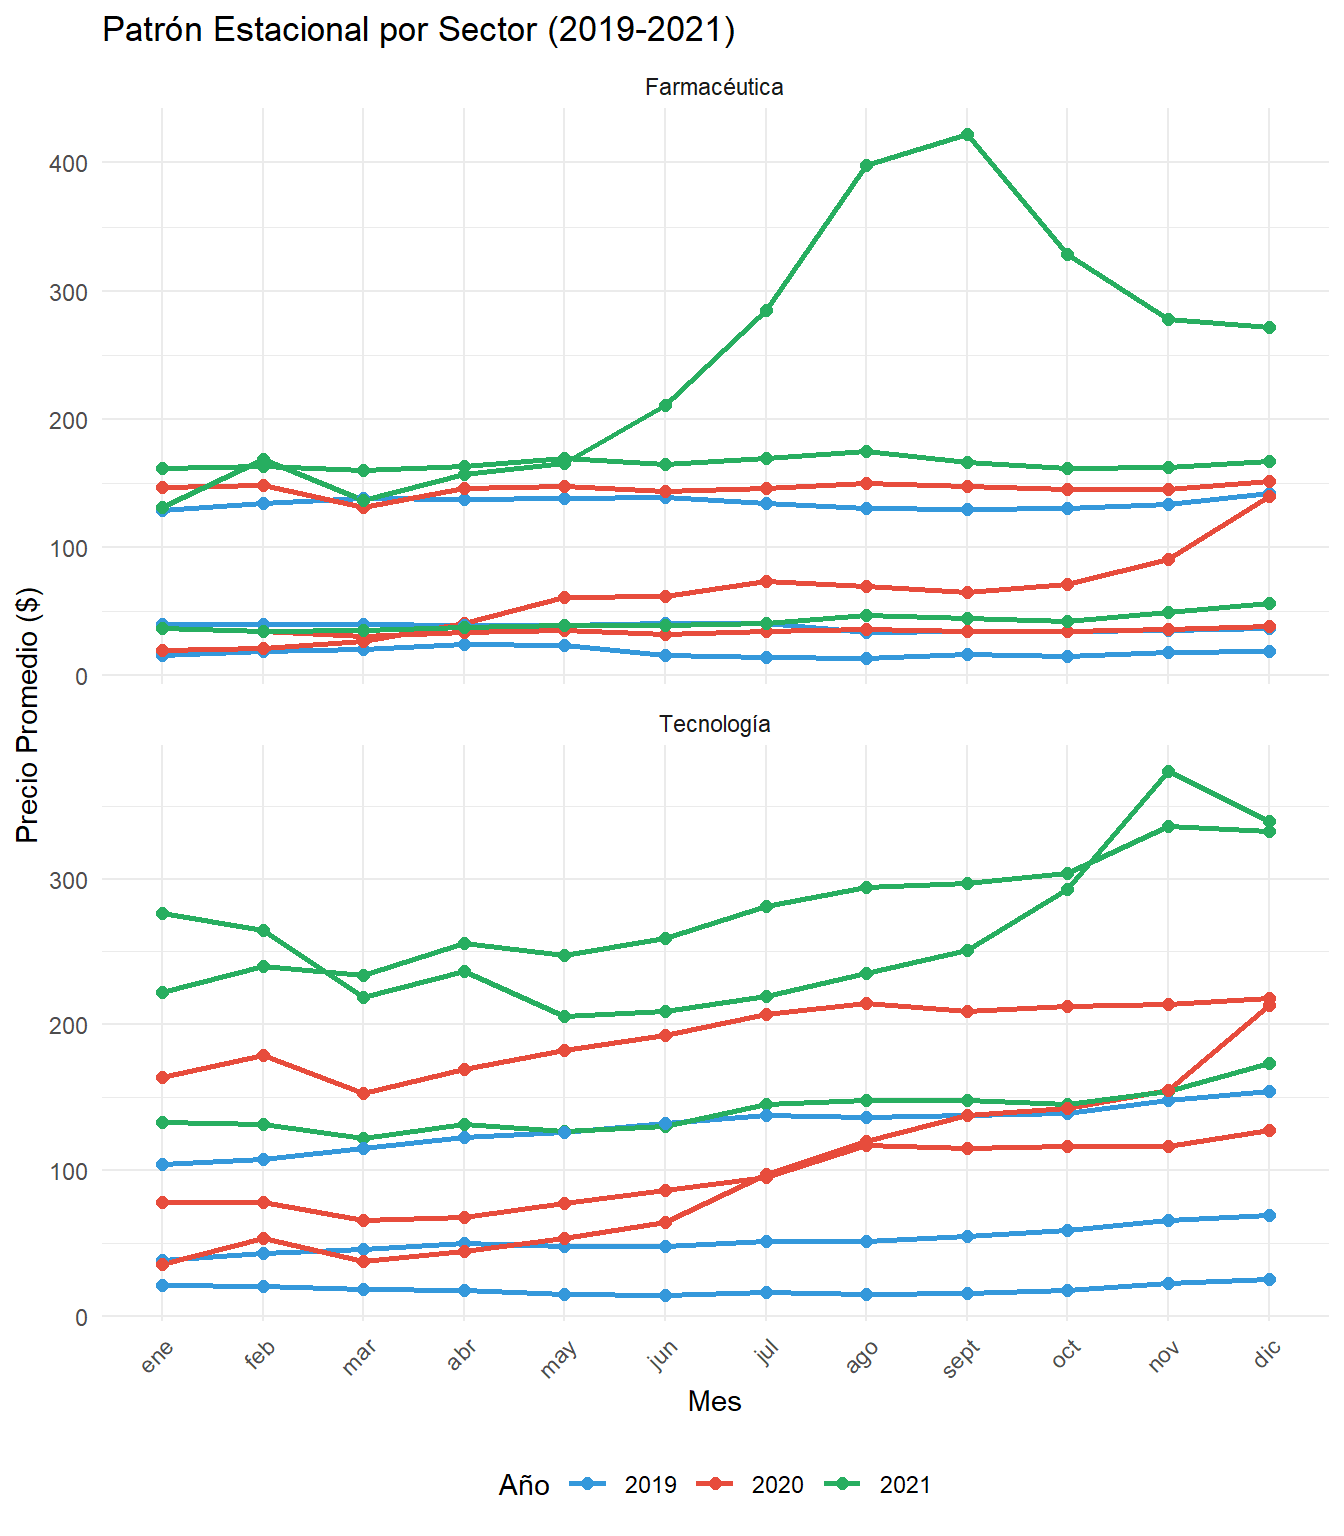
\includegraphics[keepaspectratio]{01-intro_files/figure-latex/estacionalidad-1.pdf}}
\caption{\label{fig:estacionalidad}Patrón de precios mensuales por año. Se identifica claramente el impacto COVID en marzo 2020 y la recuperación diferenciada por sector.}
\end{figure}

\textbf{Patrones estacionales identificados:}

\begin{itemize}
\item
  \textbf{Marzo 2020:} Caída drástica en todos los activos coincidiendo con el crash COVID-19.
\item
  \textbf{Noviembre-Diciembre:} Tradicionalmente meses fuertes para mercados financieros, patrón que se mantiene excepto durante 2020.
\item
  \textbf{Primer trimestre:} Generalmente muestra precios más bajos, con recuperación hacia mediados de año. Patrón interrumpido en 2020 por el COVID.
\item
  \textbf{Diferencias sectoriales:} El sector tecnológico muestra recuperación más rápida post-marzo 2020, mientras farmacéuticas tienen pico en el período de vacunas (Q4 2020 - Q1 2021).
\end{itemize}

\section{Síntesis de Visualización}\label{suxedntesis-de-visualizaciuxf3n}

Las visualizaciones revelan hallazgos clave que serán profundizados en capítulos posteriores:

\begin{enumerate}
\def\labelenumi{\arabic{enumi}.}
\item
  \textbf{Impacto COVID-19:} Claro quiebre estructural en marzo 2020 visible en todas las series.
\item
  \textbf{Divergencia sectorial:} Tecnología muestra recuperación en ``V'', mientras farmacéuticas tienen comportamiento más heterogéneo.
\item
  \textbf{Volatilidad variable:} Moderna (72\%) vs J\&J (18\%) ejemplifican el rango de comportamientos dentro del mismo sector.
\item
  \textbf{Autocorrelación limitada:} Los rezagos sugieren dependencia débil, indicando que modelos simples de persistencia no serán suficientes.
\item
  \textbf{Estacionalidad interrumpida:} El COVID-19 alteró patrones estacionales tradicionales, creando un nuevo régimen de mercado.
\end{enumerate}

Estos patrones motivan el análisis formal de series de tiempo en los capítulos siguientes.

\chapter{Literature}\label{literature}

Here is a review of existing methods.

\chapter{Methods}\label{methods}

We describe our methods in this chapter.

Math can be added in body using usual syntax like this

\section{math example}\label{math-example}

\(p\) is unknown but expected to be around 1/3. Standard error will be approximated

\[
SE = \sqrt{\frac{p(1-p)}{n}} \approx \sqrt{\frac{1/3 (1 - 1/3)} {300}} = 0.027
\]

You can also use math in footnotes like this\footnote{where we mention \(p = \frac{a}{b}\)}.

We will approximate standard error to 0.027\footnote{\(p\) is unknown but expected to be around 1/3. Standard error will be approximated

  \[
  SE = \sqrt{\frac{p(1-p)}{n}} \approx \sqrt{\frac{1/3 (1 - 1/3)} {300}} = 0.027
  \]}

\chapter{Applications}\label{applications}

Some \emph{significant} applications are demonstrated in this chapter.

\section{Example one}\label{example-one}

\section{Example two}\label{example-two}

\chapter{Final Words}\label{final-words}

We have finished a nice book.

  \bibliography{book.bib,packages.bib}

\end{document}
